
\documentclass[12pt,a4paper,oneside]{report}
\def\dedication{
  \newpage
  \thispagestyle{empty}    % No page number
  \setcounter{page}{0}
  % \addtocounter{page}{-1}
  \chapter*{}            % Required for \vfill to work
  \thispagestyle{empty}    % No page number
  \null\vfill
  \begin{center}}
\def\enddedication{\end{center}\par\vfill\newpage}

\def\abstract{
  \chapter*{Abstract}
  \addcontentsline{toc}{chapter}{Abstract}
  \relax\markboth{ABSTRACT}{ABSTRACT}}
\def\endabstract{\par\newpage}

\def\abbreviations{
  \chapter*{Abbreviations}
  \addcontentsline{toc}{chapter}{Abbreviations}
  \relax\markboth{ABBREVIATIONS}{ABBREVIATIONS}}
\def\endabstract{\par\newpage}


\def\listoffigure{
  \chapter*{List of Figures}
  \addcontentsline{toc}{chapter}{List of Figures}
\listoffigures
  \relax\markboth{List of Figures}{List of Figures}}
\def\listoffigure{\par\newpage}


\setlength{\textheight}{245mm}
\setlength{\textwidth}{160mm}

\setlength{\headheight}{6mm}
\setlength{\headsep}{12mm}
\setlength{\topmargin}{15mm}

\expandafter\def\expandafter\normalsize\expandafter{%
    \normalsize
    \setlength\abovedisplayskip{15pt}
    \setlength\belowdisplayskip{15pt}
    \setlength\abovedisplayshortskip{15pt}
    \setlength\belowdisplayshortskip{15pt}
}

\usepackage{amsmath}
\usepackage{amsthm}
\usepackage{amssymb}
\usepackage{amsmath}
\usepackage{graphicx}
\usepackage{subfigure}
\usepackage{float}
% \usepackage{epstopdf}
\usepackage{tikz}
\usetikzlibrary{intersections}
\usetikzlibrary{through}
\usetikzlibrary{angles}
\usetikzlibrary{calc}
\usetikzlibrary{quotes}
%\usepackage{hyperref}

\usepackage{caption}
\usepackage[ruled]{algorithm2e}
\usepackage[top=1in, bottom=1in, left=1in, right=1in]{geometry}
\newcommand{\oneskip}{1.0}
\newcommand{\twoskip}{1.5}
\newcommand{\singlespace}
  {\renewcommand{\baselinestretch}{\oneskip}\Large\normalsize}
\newcommand{\doublespace}
  {\renewcommand{\baselinestretch}{\twoskip}\Large\normalsize}
\usepackage{makeidx}
\usepackage{fancyhdr}
\usepackage[titletoc,page]{appendix}
% \usepackage{bm}
% \usepackage{times}
\usepackage{listings}
\usepackage{color}
\lstset{
    language=C++, 
    breaklines=true, 
    captionpos=b, 
    tabsize=2, 
    frame=single, 
    basicstyle=\footnotesize, 
    showspaces=false, 
    showstringspaces=false, 
    showtabs=true 
}

\usepackage[bottom]{footmisc}
\usepackage[colorlinks]{hyperref}
\hypersetup{
    colorlinks,%
    citecolor=black,%
    filecolor=black,%
    linkcolor= black,%
    urlcolor=black
}
\usepackage[figure,table]{hypcap}
\usepackage{verbatim}
\usepackage{pdfpages}
%\newtheorem{theorem}{Theorem}[section]
%\newtheorem{lemma}[theorem]{Lemma}
%\newtheorem{proposition}[theorem]{Proposition}
%\newtheorem{corollary}[theorem]{Corollary}

%=====================================================================
%  Single counter for theorems and theorem-like environments:
%=====================================================================
 \newtheorem{theorem}{Theorem}[chapter]
 \newtheorem{assertion}[theorem]{Assertion}
 \newtheorem{claim}[theorem]{Claim}
 \newtheorem{conjecture}[theorem]{Conjecture}
 \newtheorem{corollary}[theorem]{Corollary}
 \newtheorem{definition}[theorem]{Definition}
 \newtheorem{example}[theorem]{Example}
% \newtheorem{figger}[theorem]{Figure}
 \newtheorem{lemma}[theorem]{Lemma}
 \newtheorem{prop}[theorem]{Proposition}
% \newtheorem{remark}[theorem]{Remark}
\newcommand{\beq}{\begin{equation}}
\newcommand{\eeq}{\end{equation}}
\newcommand{\bea}{\begin{eqnarray}}
\newcommand{\eea}{\end{eqnarray}}

\linespread{2.0}
\makeindex
\begin{document}

\singlespace \begin{titlepage}
    \begin{center}
	%\large{\textbf{Dual Degree Dissertation}} \\
	%\vspace{0.25in}
	\textbf{%
	\vspace{0.05in}
	\Large{\textsc{Sojourn Time of Moving Relays in Dual-Hop Cooperative Communication}}\\ \vspace{0.1in}
	}
	\vspace{0.5in}
	\large Submitted in partial fulfillment of\\
	the requirements for the degree of\\
	\vspace{0.3in}
	\textbf{Bachelor of Technology} \\ \emph{in Electrical Engineering} \\ \& \\ \textbf{Master of Technology} \\ \emph{in Communications and Signal Processing}\\ \vspace{0.05in}

%  (under the Dual Degree Programme) \\
	\vspace{0.30in}
	\large{by}\\
	\vspace{0.30in}

	\large{\textsc{\textbf{Prudhvi Porandla}}}\\110070039

	\vspace{0.6in}
        \normalsize{Under the guidance of}\\ \vspace{0.1in}
% 	\vspace{0in}
	\textbf{\large{	Prof. S. N. Merchant
}}\\
	\vspace{0.2in}

	\begin{figure*}[h]
	\begin{center}
	
\includegraphics[width=1.8in]{images/logo.jpg}
	\end{center}
	\end{figure*}

% 	\vspace{0.1in}
	
	\vspace{-0.2in}
	\large{%
	Department of Electrical Engineering\\
 	\vspace{0.05in}
	Indian Institute of Technology Bombay\\
% 	\vspace{-0.05in}
% 	Powai, Mumbai -- 400076}\\
	% \vspace{0.2in}
	% \date{March, 2007}
	2016
	}

	\end{center}
\end{titlepage}
 \doublespace
\pagebreak
\clearpage\pagenumbering{roman}

 % This makes the page numbers Roman (i, ii, etc)

%\newpage
%\thispagestyle{empty}
%\mbox{}
% %--------------------------------------------------------------------%
% % APPROVAL SHEET
% %   - for final thesis, you need Approval Sheet. So, uncomment the
% %     \makeapproval command.
% %     it should come after dedication, if dedication is
% %     present. Otherwise it is the first page after title page.
% \makeapproval
% \thispagestyle{empty}
% \begin{center}
%   \begin{Huge}
%     \textsc{\textbf{Certificate}}
%   \end{Huge}
% \end{center}
% % \begin{center}
% % Department of Mechanical Engineering\\
% % Indian Institute of Technology Bombay
% % \end{center}
% 
% \vspace{1in}
% \begin{center}
%  Certified that this Dual Degree Project Stage-I Report titled \\ \textit{``\textbf{Next Generation Distributed Cellular Networks} \\ Architecture and Interference Management''} \\by\\Gaurav Varshney (Roll No. 07D07037) \\ is approved by me for submission. \\To the best of my knowledge, the report represents work carried out by the student.\end{center}
% 
% \vspace{1in}
% \begin{table*}[hb]
% \begin{center}
% \begin{tabular}{lr}
% Date: \hspace{1.9in} & \hspace{1.9in} \textbf{Prof. Abhay Karandikar}\\
% \end{tabular}
% \end{center}
% \end{table*}
% \end{certificate}
\newpage

\thispagestyle{empty}
\begin{center}
  \begin{Huge}
    \textsc{\textbf{Dissertation Approval}}
  \end{Huge}
\end{center}

\vspace{0.2in}

 The dissertation entitled \textit{TITLE} by \textit{Prudhvi Porandla (Roll No. 110070039)} is approved for the degree of \textit{Bachelor in Technology} in \textit{Electrical Engineering} and \textit{Master of Technology} in \textit{Communications and Signal Processing.}


\vspace{0.1in}
\begin{flushright}
\textbf{Examiners} \\
\vspace{1.5in}
\textbf{Supervisors}\\
\vspace{1.5in}
 \textbf{Chairman}\\

\end{flushright}
\vspace{0.7in}
Date :    \\
Place :\\
%\begin{table*}[hb]
%\begin{center}
%\begin{tabular}{ll}
%\textbf{Prof.  IITB} & \hspace{0.7in} \textbf{Prof. , IITB}\\
%(Internal Examiner) & \hspace{0.7in} (External Examiner)\\
%\vspace{0.5in}\\
%\textbf{Prof. Rajbabu Velmurugan, IITB} & \hspace{0.7in}  \textbf{Prof. Sibiraj Pillai, IITB} \\ 
%(Guide) & \hspace{0.7in} (Co-Guide)\\
%\vspace{0.5in}\\
%\textbf{Prof. , IITB}\\
%(Chairman)\\
%\end{tabular} \vspace{0.2in}
%\end{center}
%\begin{tabular}{ll}
%Date: & May 22, 2015 \\ \vspace{30pt}
%Place: & Indian Institute of Technology Bombay, Mumbai\\
%\end{tabular}
%
%\end{table*}

%\newpage
%\thispagestyle{empty}
%\mbox{}
%  \newpage
\newpage
\thispagestyle{empty}
\begin{center}
  \begin{Huge}
    \textsc{\textbf{Declaration}}
  \end{Huge}
\end{center}

\vspace{0.5in}

 I declare that this written submission represents my ideas in my own words and wherever others' ideas or words have been included, I have adequately cited and referenced the original sources. I also declare that I have adhered to all principles of academic honesty and integrity and have not misrepresented or fabricated or falsified any idea/ data/ fact/ source in my submission. I understand that any violation of the above will be cause for disciplinary action by IIT Bombay and can also evoke penal action from the sources which have thus not been properly cited or from whom proper permission has not been taken when needed.

\vspace{1.5in}
% \begin{table*}[hb]
% \begin{center}
\hfill \textbf{Prudhvi Porandla}\\
\noindent
\begin{tabular}{ll}
Date: & June 22, 2016\\ \vspace{30pt}
Place: & Indian Institute of Technology Bombay, Mumbai\\
\end{tabular}
% 

% \begin{dedication}
  \newpage
  \thispagestyle{empty}    % No page number

  \begin{center}  \null\vfill
   \textit{\Large To my beloved parents}
  \null\vfill
  \end{center}
% \newpage

% \end{dedication}
%\newpage
%\thispagestyle{empty}
%\mbox{}


\newpage
\thispagestyle{empty}
\begin{center}
  \begin{Huge}
    \textsc{\textbf{Acknowledgements}}
  \end{Huge}
\end{center}

\vspace{0.25in}

I would like to express my sincere gratitude to my supervisor Prof. S. N. Merchant for his invaluable guidance throughout the three years of my association with him. They have always been accessible and willing to clear my doubts and have provided valuable insights that helped me develop new ways to approach the problem and come up with better solutions.\\ %\vspace{0.2in}

\vspace{0.6in}
\noindent June 22, 2016    \hfill \textbf{Prudhvi Porandla}\\


%\newpage
%\thispagestyle{empty}
%\mbox{}


\clearpage\pagenumbering{roman} 
\begin{abstract}

We explore the application of compressed sensing for solving problems in radio astronomy where the source images are generally sparse in some domain. We obtain an incomplete set of noisy Fourier measurements of the image through the radio telescope array and the goal is to reconstruct the image by making use of the sparse nature of the images.

In this report we consider the case where we have multiple sets of Fourier measurements corresponding to different images and in addition we have some knowledge about some overlapping information between the  images. By making use of the overlapping information we should be able to perform better reconstruction than in the case where we perform the reconstruction for the images independently. 

We propose a coupled formulation where we solve a joint minimization problem to perform simultaneous recovery of multiple images. We restrict ourselves to the case where we have two images and present an alternating algorithm that solves the joint minimization problem.

We conduct experiments on different classes of images that include images that are sparse in spatial domain, images that are sparse in wavelet domain and images that are sum of a spatial domain sparse component and a wavelet domain sparse component. In all the cases we observed that the coupled formulation that does simulataneous recovery has better performance as compared to when we perform the reconstructions independently.

 \newpage

\tableofcontents

\listoffigures
  \addcontentsline{toc}{chapter}{List of Figures}
  
\clearpage\pagenumbering{arabic}
\pagestyle{fancy}
\fancyfoot{}                            % Delete current footer settings
%\fancyhf{} %clear all fields
\fancyhead[RO,LE]{\thepage}
\fancyhead[RE]{\leftmark}
\fancyhead[LO]{\rightmark}


\chapter{Introduction}
The broad goal of the field of signal processing is to reconstruct a signal and gain insights into its characteristics based on a series of sampling measurements obtained at discrete time intervals. For a general signal, this task is impossible due to non-availability of data in between two sampling intervals. But, with some prior information about the signal, measurements can be conducted in appropriate ways that enable reconstruction of signals to the desired accuracy.

For example, for a smooth signal which varies slowly with time, sample and hold type of measurements can be conducted to reconstruct the signal to the 
required accuracy.  For another category of signals namely bandlimited signals, the Nyquist-Shannon sampling theorem was an important breakthrough in the field of signal processing. The Nyquist-Shannon sampling theorem states that perfect reconstruction is possible from a set of uniformly spaced samples taken at the Nqyuist rate of twice the highest frequency present in the signal.

Unfortunately, in many applications it may be too costly or physically impossible to build devices capable of sampling at the Nyquist rate or even if it is possible we may end up with far too many samples to efficiently store and process. To address the challenges involved in dealing with such high dimensional data we often depend on compression, which aims to find the most concise representation of a signal that is able to achieve a target level of distortion. Transform coding, one of the most popular techniques for signal compression, relies on finding a basis or a frame that provides sparse or compressible representations for signals in a class of interest. Both sparse and compressible signals can be represented with high fidelity by preserving only the the values and locations of the largest $k$ coefficients of the signals, where $k \ll n$, and $n$ is the length of the signal.

Compressed sensing is a framework for signal acquisition and sensor design that enables a potentially large reduction in the sampling and computation costs for sensing signals that have a sparse or compressible representation. The fundamental idea behind compressed sensing is rather than first sampling at a higher rate and then compressing sampled data, we would like to directly sense the data in compressed form at a much lower sampling rate. The field of compressed sensing grew out of the work of  Candes, Tao and Romberg who showed that, a finite-dimensional signal having a sparse or compressible representation can be recovered from a much smaller number of linear measurements than what Nyquist rate sampling demands \cite{candes,Tao,romberg}. Compressed sensing methods are fast and highly configurable, which makes them highly attractive for a lot of problems such as 
improving MRI imaging \cite{Tao}, developing single pixel cameras \cite{single_pixel}, face recognition algorithms etc. However compressed sensing is still a recent field and its applicability to a large number fields has not yet been fully studied.
Basic information on compressed sensing can be obtained from \cite{cs_rice}. For a complete up-to-date review on compressed sensing refer to \cite{cs_book}. As a part of this thesis, we study the application of compressed sensing methods for improving radio astronomy imaging techniques.

\section*{Compressed Sensing and Radio Astronomy}
Radio Astronomy studies celestial objects at radio frequencies around the metre wavelength, by utilizing the techniques of radio interferometry and aperture synthesis. Mathematically, the problem is equivalent to reconstructing the image of the astronomical object from incomplete and noisy Fourier measurements of the image. From the theory of compressed sensing we know that such measurements may actually suffice for accurate reconstruction of the image provided that the image is sparse in some domain.

Our earlier work \cite{stage1} focused on applying compressed sensing techniques to recover an image of astronomical sources from a an incomplete set of its Fourier measurements. Also, we analyzed the optimality of the GMRT telescope \cite{GMRT} with respect to reconstruction using compressed sensing techniques and came up with optimal antenna locations for additions to the array. 

In this project we consider the case where we have two sets of Fourier measurements corresponding to two different images but in addition we have knowledge about some overlapping information between the two images. The goal is to use this additional information and perform  simultaneous recovery of both images that performs better than if we reconstruct the images independently.  We propose an alternating algorithm that performs simultaneous recovery by solving a joint minimization problem and then conduct experiments to compare the results of the alternating algorithm with those obtained from independent reconstructions. 



\section*{Organization of the report}
The organization of the report is as follows:
\begin{enumerate}

	\item \textbf{Chapter 2} introduces radio astronomy and the basics of radio imaging techniques such as radio interferometry and aperture synthesis.

	\item \textbf{Chapter 3} presents the mathematical model for the compressed sensing problem in a simultaneous recovery setting. We present an alternating algorithm to solve the joint minimization problem to perform simultaneous recovery.

	\item \textbf{Chapter 4} Absorbing MC

	\item \textbf{Chapter 5} analyzes the experiments conducted on simulated data. In this chapter the performance of the alternating algorithm that performs simultaneous recovery is compared against that of the algorithm that reconstructs images separately.

	\item \textbf{Conclusion and Further Work}

\end{enumerate}



\chapter{Relaying and Cooperation Policies}
This chapter is heavily based on the published work \cite{elk} of Hussain Elkotby and Mai Vu of Tufts University. Analysis and simulations of their work was done during first phase of the project to gain insights into signal design of various relaying schemes and to learn about the ways in which cellular networks are modelled and analysed, what challenges user-assisted relaying presents. The only subject in this chapter that will be useful for the later part of this report is presented in section \ref{sec:downcoop}.   

\section{Partial Decode-and-Forward Relaying}
In this section, we discuss the signal design, channel model and achievable rate of PDF relaying scheme.
\subsection{Signal Design}
Consider a source $\mathcal{S}$, its relay $\mathcal{R}$ and the destination $\mathcal{D}$. Each transmission block is divided into two phases: 1. broadcast transmission in which $\mathcal{S}$ broadcasts to both $\mathcal{R}$ and $\mathcal{D}$. 2. multiple access transmission in which both $\mathcal{S}$ and $\mathcal{R}$ transmit to $\mathcal{D}$. In each block of transmission, $\mathcal{S}$ splits its information into a common part and a private part. The common part is encoded via $U_s^b$ in the 1st phase and $U_s^{m_1}$ in the 2nd phase; and the private part is encoded via $V_s^{m_2}$ in the 2nd phase. The relay $\mathcal{R}$ decodes the information sent by $\mathcal{S}$ in first phase and encodes the same information using $U_s^{m_1}$ in the 2nd phase. \\ 

\begin{figure}[h]
	\centering \vspace{-0.1in}
	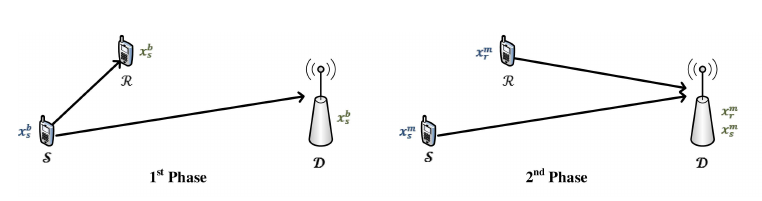
\includegraphics[height = 2in,width=5in,angle=00]{images/pdfRelaying.png}
	\vspace{-20pt} 
	\caption[Transmission phases in PDF relaying]{\small Transmission phases in PDF relaying\footnotemark}
	\label{fig:sysModel}
\end{figure}
\footnotetext{Image Source: \cite{elk} Hussain Elkotby}
The signals transmitted by $\mathcal{R}$ and $\mathcal{S}$ are as follows:
\begin{align}
\text{Phase 1:}\quad x^b_s &= \sqrt{P_s^b} U_s^b, \label{eq:tranSig1}\\
\text{Phase 2:}\quad x_r^m &= \sqrt{P_r^m}U_s^{m_1}, \label{eq:tranSig2}\\ 
 x^m_s &= \sqrt{P_s^{m_1}}U_s^{m_1} + \sqrt{P_s^{m_2}}V_s^{m_2} \label{eq:tranSig3}
\end{align}
All codewords above are picked from independent Gaussian codebooks with zero mean and unit variance. \\ \\
\textbf{Power Constraints:} Let $P_s$ and $P_r$ be the transmit powers of $\mathcal{S}$ and $\mathcal{R}$ respectively and $\alpha_1$ be the fraction of transmission time allocated to first phase, then the following average power constraints should to be satisfied:
\begin{equation}
\alpha_1 P_s^b + \alpha_2 P_s^m = P_s,\quad \alpha_2P_r^m = P_r
\end{equation}
where $\alpha_2 = 1-\alpha_1$

\subsection{Channel Model}
Considering the transmit signals presented above and assuming flat fading over the two phases, the received signals at $\mathcal{R}$ and $\mathcal{D}$ during first phase are 
\begin{equation}
Y_r^b = h_{sr}x^b_s + Z_r^b , \quad Y_d^b = h_{sd}x^b_s + Z_d^b
\end{equation}
where $b$ denotes broadcast mode, $Z_r^b$ and $Z_d^b$ are \textit{i.i.d} circularly-symmetric complex gaussians with mean 0 and variance $\sigma^2$  - $\mathcal{CN}(0,\sigma^2)$ that represent noises at $\mathcal{R}$ and $\mathcal{D}$. \\
Similarly the received signal at $\mathcal{D}$ during second phase can be modelled as 
\begin{equation}
Y_d^m = h_{sd}x^m_s + h_{rd}x_r^m + Z_d^m
\end{equation}
here $m$ denotes multicast transmission; all others have usual meaning.
The above expression is true only if $\mathcal{D}$ has knowledge about the phase offset between $\mathcal{S}$ and $\mathcal{R}$. This assumption is justified by noting that the phase offset between the two nodes can be estimated at base station.

\subsection{Achievable Rate}
With transmit signals in equations~\ref{eq:tranSig1}-\ref{eq:tranSig3} and joint ML decoding rule at $\mathcal{D}$, the achievable rate for this relaying scheme is:
\begin{equation} \label{eq:rate}
R_{PDF} \leq min(C_1+C_2,C_3)
\end{equation}
\begin{align}
\text{where } C_1 &= \alpha_1 \log\Big(1+|h_{sr}|^2P_s^b\Big),\\
C_2 &= \alpha_2 \log\Big(1+|h_{sd}|^2P_s^{m_2}\Big),\\
C_3 &= \alpha_1 \log\Big(1+|h_{sd}|^2P_s^b\Big) + \alpha_2\log\bigg(1+|h_{sd}|^2P_s^{m_2} + \Big(|h_{sd}|\sqrt{P_s^{m_1}} + |h_{rd}|\sqrt{P_r^m}\Big)^2\bigg)
\end{align}
$C_1$ represents the rate of the common part that can be decoded at $\mathcal{R}$, $C_2$  the private part that can be decoded at $\mathcal{D}$ provided the common part has been decoded correctly, and $C_3$ both the common and private parts that can be jointly decoded at $\mathcal{D}$. These rates are achievable provided full CSI at all receivers and the source-relay phase offset knowledge.
\par
Now that we know what PDF relaying scheme is and the achievable rate, let us see how this scheme performs in cellular networks. To analyse system performance under PDF relaying, we need to know network geometry i.e., how the users and base stations are distributed, how many users can take advantage of relaying, how users identify a potential relay etc. In the next couple of sections we describe network geometry,  received signals and interference model when relaying is deployed in the whole network, and cooperation policies.

\section{Cellular Network Geometry and User-Assisted Relaying}

\subsection{Network geometry model}
Consider a cellular system which consists of multiple
cells, each cell has a single base station and each base station
serves multiple users. Each of the users uses a distinct frequency
block. Each user is served by the single base station that
is closest to that user.


\par We use stochastic geometry to
describe the uplink cellular network. We
assume that the active users in different cells that use the same resource block and cause interference to each other are distributed on a two-dimensional plane according to a homogeneous and stationary Poisson point process (PPP)
$\Phi_1$ with intensity $\lambda_1$. The set of user equipments(UEs) that are in idle state and can participate in relaying are distributed according to another PPP $\Phi_2$ with intensity $\lambda_2$. We assume $\Phi_1$ and $\Phi_2$ are independent. Furthermore, under the assumption that each BS serves a
single mobile in a given resource block, the BS should be closer to its served UE than to any other UE. Therefore we assume each BS is uniformly distributed in the Voronoi cell of its served UE. Fig.~\ref{fig:netLayout} shows an example layout of the network.

\begin{figure}[h]
	\centering \vspace{-0.1in}
	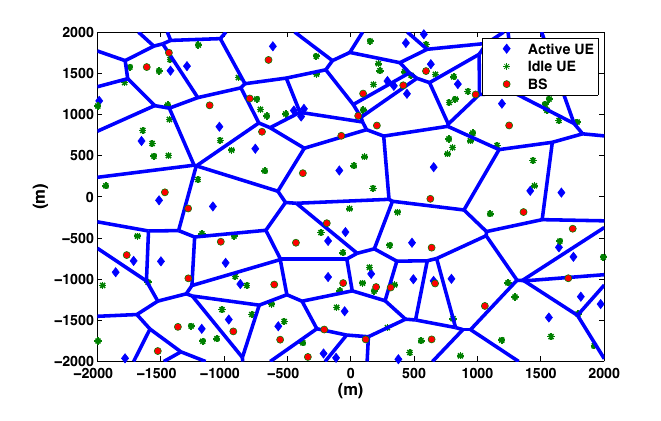
\includegraphics[height = 3in,width=4in,angle=00]{images/netLayoutPaper.png}
	\vspace{-20pt} 
	\caption[Sample layout of a cellular network ($\lambda_2 = 2\lambda_1$)]{\small  Sample layout of a cellular network ($\lambda_2 = 2\lambda_1$) \footnotemark}
	\label{fig:netLayout}
\end{figure}
\footnotetext{Image Source: \cite{elk} Hussain Elkotby}


\subsection{Channel Model}
In this section, we describe the channel model when PDF relaying is deployed in cellular network. In this case, there will be out-of-cell inteference in addition to noise. The interference is due to frequency reuse in other cells.
\par Consider $i^{th}$ active UE, we model the received signals at the relay and base station in this cell during 1st phase as
\begin{equation*}
Y_{r,i}^b = h^{(i)}_{sr}x_{s,i}^b + I_{r,i}^b + Z_{r,i}^b,
\end{equation*}
\begin{equation}
Y_{d,i}^b = h^{(i)}_{sd}x_{s,i}^b + I_{d,i}^b + Z_{d,i}^b
\end{equation}
where $I_{r,i}^b$ and $I_{d,i}^b$ represent the interference received at the $i^{th}$ relay and destination. 
\par 
In second phase of the transmission, the received signal at the BS can be modelled as 
\begin{equation}
Y_{d,i}^m = h^{(i)}_{sd}x_{s,i}^m + h^{(i)}_{rd}x_{r,i}^m+ I_{d,i}^m + Z_{d,i}^m
\end{equation}

\subsection{Interference}
To model interference, we assume prefect frame synchronization. LTE-Advanced imposes very strict requirements on synchronization anyway. Interference at the relay during first phase and at the destination(BS) during first and second phases can be expressed as
\begin{equation*} 
I_{r,i}^b = \sum_{k \neq i} B_k h^{(k,i)}_{sr} x_{s,k}^b + (1-B_k)h_{sr}^{(k,i)}x_{s,k} ,
\end{equation*}
\begin{equation*}
I_{d,i}^b = \sum_{k \neq i} B_k h_{sd}^{(k,i)} x^b_{s,k} + (1-B_k)h_{sd}^{(k,i)}x_{s,k},
\end{equation*}
\begin{equation} \label{eq:interferences}
I_{d,i}^m = \sum_{k \neq i} B_k \Big(h_{sd}^{(k,i)} x^m_{s,k} + h_{rd}^{(k,i)} x^m_{r,k}\Big) + (1-B_k)h_{sd}^{(k,i)}x_{s,k}
\end{equation}
the summation is over all active users. Here, $h_{sd}^{(k,i)}$ and $h_{rd}^{(k,i)}$ , respectively, are the channel fading from the $k^{th}$ active UE in $\Phi_1$ and the associated relaying UE in $\Phi_2$ to the BS associated with the $i^{th}$ active UE in $\Phi_1$; and $h_{sr}^{(k,i)}$ is the channel fading from the $k^{th}$ active UE in $\Phi_1$ to the relaying UE associated with the $i^{th}$ active UE in $\Phi_1$.
\par $B_k$ in above expressions is a Bernoulli random variable with success probability $\rho$. $B_k = 1$ is used to indicate the $k^{th}$ active UE's decision to exploit the help of another idle UE, a relay, and apply the relaying transmission strategy, and $B_k = 0$ indicates that the $k^{th}$ UE has no relay. In section~\ref{sec:coop}, we derive the cooperation probability $\rho$ for different cooperation policies.
\par
 For a given setting of nodes locations, based on the
interference model in Eq.~\ref{eq:interferences}, we can use the fact
that interference at either the relay or destination is the
sum of an infinite number of signals undergoing independent fading from nodes distributed in the infinite 2-D plane and use the law of large numbers to approximate the interference as a complex Gaussian distribution.
Also, since the transmitted codewords are complex Gaussian with zero mean, mean of interference is zero. To fully characterize interference as a
complex Gaussian distribution, we define their distributions as $ I_{d,i}^b \sim \mathcal{CN} (0,\mathcal{Q}_{d,i}^b), I_{d,i}
^m \sim \mathcal{CN}(0,\mathcal{Q}_{d,i}^m),$ and $I_{r,i}^b \sim \mathcal{CN}
(0,\mathcal{Q}_{r,i})$ with the variances derived later
in Section~\ref{sec:interference}. The power of these interference terms which
correspond to the variance of the Gaussian random variables
are function of node locations and hence vary with different
network realizations.

\subsection{Equivalent Standard Channel Model}
Using the interference model discussed above, we can convert the channel model in case of relaying into the standard form to capture the effects of
interference into the channel fading as
\begin{align*}
\tilde{Y}_{r,i}^b &= \tilde{h}_{sr}^{(i)}x_{s,i}^b + \tilde{Z}_{r,i}^b, \\
\tilde{Y}_{d,i}^b &= \tilde{h}_{sd}^{(i)}x_{s,i}^b + \tilde{Z}_{d,i}^b, \\
\tilde{Y}_{d,i}^m &= \tilde{h}_{sd}^{(i)}x_{s,i}^m + \tilde{h}_{rd}^{(i)}x_{r,i}^m + \tilde{Z}_{d,i}^m
\end{align*}
where the new channel fading terms are defined as

\begin{equation*}
\tilde{h}_{sr}^{(i)} = \frac{h_{sr}^{(i)}}{\sqrt{\mathcal{Q}_{r,i} + \sigma^2}}, \quad \tilde{h}_{sd}^{(b,i)} = \frac{h_{sd}^{(i)}}{\sqrt{\mathcal{Q}_{d,i}^b + \sigma^2}} \quad
\tilde{h}_{sd}^{(m,i)} = \frac{h_{sd}^{(i)}}{\sqrt{\mathcal{Q}_{d,i}^m + \sigma^2}},
\quad \tilde{h}_{rd}^{(i)} = \frac{h_{rd}^{(i)}}{\sqrt{\mathcal{Q}_{d,i}^m + \sigma^2}}
\end{equation*}
and the noise terms are now all $\mathcal{CN}(0,1)$. Using these equivalent 
standard channels, we can compute the transmission rate using Eq.~\ref{eq:rate}

\section{Cooperation Policies and Probability} \label{sec:coop}
In this section, we look at three cooperation policies: an ideal policy $E_1$, a 
pure geometric policy $E_2$ and a hybrid policy $E_3$ that defines whether an active UE should select an inactive UE to use it in PDF relaying. Also, expressions for cooperation probabilities of $E_2$ and $E_3$ are derived.
\subsection{Policies}
\subsubsection{Ideal Policy $E_1$}
The ideal cooperation policy $E_1$ requires the active UE nodes to know instantaneous  SINRs of the relay link($\mathcal{S}-\mathcal{R}$) and the
direct link($\mathcal{S}-\mathcal{D}$). The policy is defined as 
\begin{align*}
E_1 &= \Big\{|\tilde{h}_{(sr)}^{(k)}|^2 \geq |\tilde{h}_{(sd)}^{(k)}|^2\Big\} \\
&\backsimeq \Big\{ \frac{g_{sr}r_2^{-\alpha}}{\mathcal{Q}_{r,k}} \geq \frac{g_{sd}r_1^{-\alpha}}{\mathcal{Q}_{d,k}^b} \Big\}
\end{align*}
where $r_1$ and $r_2$ denote the direct distance
between $\mathcal{S}$ and $\mathcal{D}$ and cooperation distance between $\mathcal{S}$ and its closest idle UE, respectively and $\alpha$ is pathloss exponent. This event $E_1$ identifies whether an idle UE will be associated as a relay for the $k^{th}$ UE and participate in transmission. Noise variance $\sigma^2$ is ignored since interference power dominates. 
\par Since interference at relay and destination during first phase is more or less the same and $g_{sr}, g_{sd}$ are identically distributed, we can safely ignore them and propose a policy that depends only on distances.

\subsubsection{Pure Geometric Policy $E_2$}
This policy is defined as
\begin{equation}
E_2 = \{r_2\leq r_1, D \leq r_1 \}
\end{equation}
where $D$ is the distance between $\mathcal{R}$ and $\mathcal{D}$. In words, if source's(active UE's) nearest idle neighbour is in the intersection region of two circles of radius $r_1$ centered at source and destination, then that idle UE will be chosen to act as a relay.
\par $E_2$ is more practical than policy $E_1$ in the sense that
it does not require full knowledge of both the channel fading
and the interference at the decision making node. Instead, it
only requires the decision making nodes to know the distances
from the active user to the nearest idle user and to the base
station. It represents a practical decision making strategy for
fast fading channels, requiring no knowledge of the channel
fading. 
\subsubsection{Hybrid Policy $E_3$}
This policy is proposed for slow fading channels where small scale fading parameters estimation and their
feedback to the decision making node is feasible. 
\begin{equation}
E_3 = \{g_{sd}r_1^{-\alpha} \leq g_{sr}r_2^{-\alpha}, D \leq r_1 \}
\end{equation}
Note that this cooperation policy is still independent of the
interference as in the pure geometric cooperation policy $E_2$.

\subsection{Cooperation Probabilities}
In this part of the section we derive cooperation probabilities $\rho_2$ and $\rho_3$ for the policies $E_2$ and $E_3$ respectively. For the ideal policy $E_1$, analytic evaluation of the
cooperation probability is rather complicated because of the
inter-dependency between the cooperation decision and consequential interference among different cells. Consider a random BS and its associated active UE. 
The distribution of the distance
$r_1$ between the $i^{th}$ UE and its associated BS can be shown to
be Rayleigh distributed directly from the null probability of a
two dimensional PPP distribution. 
\par  Due to the stationarity of the
PPP, i.e., location of the origin doesn't change the distribution of points, and the independence of $\Phi_2$ from BSs distribution we can assume that
the location of the UE associated with the BS under study
represents the origin point of $\Phi_2$ . Then, each UE
in $\Phi_1$ chooses the closest UE in $\Phi_2$ to assist it in relaying
its message to the serving BS. Hence, similar to source-to-
destination distance, the distribution of the source-to-relay
distance $r_2$ between the $i^{th}$ UE and its associated relaying UE
can be also shown to be Rayleigh distributed from the null probability of a two dimensional PPP. Therefore,
\begin{equation*}
f_{r_1}(r_1) = 2\pi\lambda_1r_1e^{-\lambda_1\pi r_1^2},
\end{equation*}
\begin{equation}
f_{r_2}(r_2) = 2\pi\lambda_2r_2e^{-\lambda_2\pi r_2^2}
\end{equation}

\begin{theorem}{Cooperation Probabilities.}
The probability of
deploying user-assisted relaying for a randomly located active
user within a cell can be evaluated as follows:
\begin{itemize}
\item[i.] For policy $E_2$
\begin{equation}
\rho_2 = \int_{-\pi/2}^{-\pi/3}\frac{2\lambda_2 cos^2\psi_0}{\pi(\lambda_1+4\lambda_2cos^2\psi_0)}d\psi_0 + \int_{\pi/3}^{\pi/2}\frac{2\lambda_2 cos^2\psi_0}{\pi(\lambda_1+4\lambda_2cos^2\psi_0)}d\psi_0 + \frac{\lambda_2}{3(\lambda_1+\lambda_2)}
\end{equation}
\item[ii.] For policy $E_3$
\begin{align*}
\rho_3 &= \int_0^2 f_{\beta}(z)\int_{-\pi/2}^{-cos^{-1}(z/2)}\frac{2\lambda_2 cos^2\psi_0}{\pi(\lambda_1+4\lambda_2cos^2\psi_0)}d\psi_0 dz \\ 
&+ \int_0^2 f_{\beta}(z)\int^{\pi/2}_{cos^{-1}(z/2)}\frac{2\lambda_2 cos^2\psi_0}{\pi(\lambda_1+4\lambda_2cos^2\psi_0)}d\psi_0 dz \\ &+\int_0^2 f_{\beta}(z)\frac{\lambda_2 z^2 cos^{-1}(z/2)}{\pi(\lambda_1+\lambda_2z^2)}dz \\ 
&+ \int_2^{\infty} f_{\beta}(z)\int_{-\pi/2}^{\pi/2}\frac{2\lambda_2 cos^2\psi_0}{\pi(\lambda_1+4\lambda_2cos^2\psi_0)}d\psi_0 dz
\end{align*}
where $\beta = \bigg(\frac{g_{sr}}{g_{sd}}\bigg)^{1/\alpha}$ and $f_{\beta}(z)$ is pdf of $\beta$ which can be shown to be 
\begin{equation}
f_{\beta}(z) = \frac{\alpha z^{\alpha-1}}{(1+z^{\alpha})^2}
\end{equation}
\end{itemize}
\end{theorem}
\begin{proof}
\begin{itemize}
\item[i.] 
\begin{align*}
\rho_2 &= \mathbb{P}\{E_2\} \\
&= \mathbb{P}\{r_2 \leq r_1, r_1^2+r_2^2-2r_1r_2cos\psi_0 \leq r_1^2\} \\
&= \mathbb{P}\{r_2 \leq r_1, r_2 \leq 2 r_1 cos\psi_0 \} \\
\end{align*}
when $|\psi_0|<\pi/3, ~ r_1 < 2r_1cos\psi_0  \Rightarrow \text{ if } r_2 < r_1 \text{, $r_2$ satisfies both inequalities.}$ Accordingly, we define $\mathcal{E}_1$ and $\mathcal{E}_2$ as follows
\begin{align*}
\mathcal{E}_1 &= (2\pi)^2\lambda_1 \lambda_2 \int_0^\infty \int_0^{2r_1 cos\psi_0}r_1r_2e^{-\pi(\lambda_1 r_1^2 + \lambda_2 r_2^2)}dr_2 dr_1 \\
&= \frac{2\lambda_2 cos^2\psi_0}{\pi(\lambda_1+4\lambda_2cos^2\psi_0)} \\
\mathcal{E}_2 &= (2\pi)^2\lambda_1 \lambda_2 \int_0^\infty \int_0^{r_1}r_1r_2e^{-\pi(\lambda_1 r_1^2 + \lambda_2 r_2^2)}dr_2 dr_1 \\
&= \frac{\lambda_2}{2\pi(\lambda_1+\lambda_2)}
\end{align*}
 
\begin{align*}
\text{Now, }\rho_2 &= \int_{-\pi/3}^{\pi/3} \mathcal{E}_2 d\psi_0 + 2\int_{\pi/3}^{\pi/2} \mathcal{E}_1d\psi_0 \\
&=  \frac{\lambda_2}{3(\lambda_1+\lambda_2)} + 2\int_{\pi/3}^{\pi/2} \mathcal{E}_1d\psi_0
\end{align*} 

\item[ii.]
\begin{align}
\rho_3 &= \mathbb{P}\{E_3\} \\
&= \mathbb{P}\{r_2 \leq \bigg(\frac{g_{sr}}{g_{sd}} \bigg)^{1/\alpha}r_1, r_1^2+r_2^2-2r_1r_2cos\psi_0 \leq r_1^2\} \\
&= \mathbb{P}\{r_2 \leq \beta r_1, r_2 \leq 2 r_1 cos\psi_0 \} \\
&= \mathbb{P}\{r_2 \leq 2 r_1 cos\psi_0 \} \qquad \text{ for } \beta > 2 \\
&= \mathbb{P}\{r_2 \leq \beta r_1\} \qquad \text{ for } \beta < 2  \text{ and } |\psi_0| < cos^{-1}(\beta/2) \\
&= \mathbb{P}\{r_2 \leq 2 r_1 cos\psi_0 \} \qquad \text{ for } \beta < 2 \text{ and } cos^{-1}(\beta/2) < |\psi_0| <  \pi/2 \\
\therefore \rho_3&= 2 \int_0^2 f_{\beta}(z)\int^{\pi/2}_{cos^{-1}(z/2)}\mathcal{E}_1 d\psi_0 dz +\int_0^2 f_{\beta}(z)\int_{-cos^{-1}(z/2)}^{cos^{-1}(z/2)}\mathcal{E}_3 d\psi_0dz \\&+ \int_2^{\infty} f_{\beta}(z)\int_{-\pi/2}^{\pi/2}\mathcal{E}_1 d\psi_0 dz \label{eq:corrected}
\end{align}

$\mathcal{E}_1$ is defined in part i. of the proof and  $\mathcal{E}_3 = \frac{\lambda_2 z^2}{2\pi(\lambda_1+\lambda_2z^2)}$ which is nothing but $\mathcal{E}_2$ with $\lambda_2 = \lambda_2z^2$. $f_\beta(z)$, the pdf of $\beta$, can be obtained as follows

\begin{align*}
F_\beta(z) &= \mathbb{P}\bigg\{ \bigg( \frac{x_1}{x_2}\bigg)^{1/\alpha} \leq z \bigg\} = \mathbb{P} \{ x_1\leq z^\alpha x_2\} \\
&= \int_0^\infty \int_0^{z^\alpha x_2} e^{-(x_1+x_2)} dx_1dx_2 \quad \text{ since } g_{sr},g_{sd} \sim Exp(1) \\
&= 1-\frac{1}{1+z^\alpha}, \qquad z \in [0,\infty)
\end{align*}
The pdf $f_\beta(z)$ is then obtained by differentiating $F_\beta(z)$ :
\begin{equation*}
    f_\beta(z) = \frac{dF_\beta(z)}{dz} = \frac{\alpha z^{\alpha-1}}{(1+z^\alpha)^2} \quad z \in [0,\infty)
\end{equation*}
\end{itemize}
\end{proof}
\section{Interference Analysis} \label{sec:interference}
User-assisted relaying actually increases the amount of out-
of-cell interference in the network as some idle users are now
transmitting when relaying information of active users. It is
therefore necessary to understand this out-of-cell interference
power, particularly its distribution, in order to assess the overall
impact of user-assisted relaying on system performance.
\subsection{First Two Moments of Interference Power} Since it is difficult to describe the
exact distribution of out-of-cell interference power, here we
choose to model the interference power to the cell under study
as a Gamma distribution by fitting the first two moments of
the interference power analytically developed using stochastic
geometry of the field of interferers outside that cell.
The expressions for interference power can be developed from Eqs.~\ref{eq:interferences}. 
\begin{align}
\mathcal{Q}_{d,i}^b &= \sum_{k\neq i}B_k \Big |h_{sd}^{(k,i)}\Big|^2P_{s,k}^b + (1-B_k)\Big|h_{sd}^{(k,i)}\Big|^2P_{s,k} \\
\mathcal{Q}_{d,i}^m &= \sum_{k\neq i}\bigg[B_k\bigg(\Big|h_{sd}^{(k,i)}\Big|^2 P_{s,k}^m+\Big|h_{rd}^{(k,i)}\Big|^2 P_{r,k}^m\bigg)\bigg] + (1-B_k) \Big| h_{sd}^{(k,i)}\Big|^2 P_{s,k} \\
\mathcal{Q}_{r,i} &= \sum_{k\neq i}B_k \Big|h_{sr}^{(k,i)}\Big|^2P_{s,k}^b + (1-B_k)\Big|h_{sr}^{(k,i)}\Big|^2P_{s,k} 
\end{align}
\begin{theorem}{Interference Power Statistics} \label{theorem:theorem2}
For network-wide
deployment of user-assisted relaying, the out-of-cell interfer-
ence generated at the destination BS and the relaying UE have
the following statistics:

\begin{itemize}
\item[i.] 
The first two moments, mean and variance, of interference
power at the destination BS during the 1st and 2nd phase,
respectively, are
\begin{equation}
\mathbb{E}[\mathcal{Q}_{d,i}^b] = \frac{2\pi\lambda_1\zeta_1}{\alpha-2}R_c^{2-\alpha}, \qquad \mathbb{E}[\mathcal{Q}_{d,i}^m] = \frac{2\pi\lambda_1\zeta_3}{\alpha-2}R_c^{2-\alpha}
\end{equation}
\begin{equation}
\text{var}[\mathcal{Q}_{d,i}^b] = \frac{\pi\lambda_1\zeta_2}{\alpha-1}R_c^{2(1-\alpha)}, \qquad \text{var}[\mathcal{Q}_{d,i}^m] = \frac{\pi\lambda_1\zeta_4}{\alpha-1}R_c^{2(1-\alpha)}
\end{equation}

\item[ii.]
The first two moments, mean and variance, of interfer-
ence power at the idle UE associated as a relay with the ith
active UE are
\begin{equation}
\mathbb{E}[\mathcal{Q}_{r,i}] = \lambda_1\zeta_1 \int_0^{2\pi}\int_{R_c}^\infty (r^2+D^2-2rDcos\theta)^{\alpha/2}rdrd\theta
\end{equation}
\begin{equation}
\text{var}[\mathcal{Q}_{r,i}] = \lambda_1\zeta_2 \int_0^{2\pi}\int_{R_c}^\infty (r^2+D^2-2rDcos\theta)^{\alpha/2}rdrd\theta
\end{equation}

\begin{align} \label{eq:zeta1}
\text{where} \quad  \zeta_1 &= \rho_1 P_{s,k}^b +(1-\rho_1)P_{s,k} \\
                \zeta_2 &= 2[\rho_1(P_{s,k}^b)^2 + (1-\rho_1)P_{s,k}^2],\\
                \zeta_3 &= \rho_1 (P_{s,k}^m+P_{r,k}^m) +(1-\rho_1)P_{s,k}, \\
                \zeta_4 &= 2[\rho_1(P_{s,k}^m+P_{r,k}^m)^2 + (1-\rho_1)P_{s,k}^2 -\rho_1P_{s,k}^mP_{r,k}^m] \label{eq:zeta4}
\end{align}
\end{itemize}
\end{theorem}
\begin{proof}
\begin{align*}
\mathbb{E}[\mathcal{Q}_{d,i}^b] &= -\frac{\partial\mathcal{L}_{\mathcal{Q}_{d,i}^b}(s)}{\partial s}\bigg\rvert_{s=0}, \\
\text{var}[\mathcal{Q}_{d,i}^b] &= -\frac{\partial^2\mathcal{L}_{\mathcal{Q}_{d,i}^b}(s)}{\partial s^2}\bigg\rvert_{s=0} - \Big(\mathbb{E}\big[\mathcal{Q}_{d,i}^b \big] \Big)^2
\end{align*}
where $\mathcal{L}_{\mathcal{Q}_{d,i}^b}(s)$ is the Laplace transform of $\mathcal{Q}_{d,i}^b$ and $R_c = 1/2\sqrt{\lambda_1}$ is the cell radius. Means and variances of $\mathcal{Q}_{d,i}^m$, $\mathcal{Q}_{r,i}$ can be calculated similarly.
\end{proof}
\par From the above results for interference power statistics, the interference power is directly proportional to both
the active users density, $\lambda_1$ , and the transmission power levels
represented by $\zeta_i , i \in [1:4] $ in Eqs.~\ref{eq:zeta1} - ~\ref{eq:zeta4}

\subsection{Modelling Interference Power Distribution}
A parameterized probability distribution, which includes a
wide variety of curve shapes, is useful in the representation of
data when the underlying model is unknown or difficult to obtain in closed form. A parameterized probability distribution is
usually characterized by its flexibility, generality, and simplicity. Although distributions are not necessarily determined by
their moments, the moments often provide useful information
and are widely used in practice. It is shown that the Gamma
distribution is a good approximation for the interference when
the point under study is closer to the cell center, but fails
to represent the actual interference distribution whenever the
point under study is exactly at the cell edge. We use the same
approach here and match a Gamma distribution to the first
two moments of the interference power terms derived earlier
in Theorem~\ref{theorem:theorem2}.
\subsubsection{Gamma Distribution}
The Gamma distribution is specified by a shape parameter $k$ and a scale parameter $\theta$. The pdf of a Gamma distributed RV $\gamma[k,\theta]$ is defined as 
\begin{equation*}
F_\gamma(q|k,\theta) = \frac{q^{k-1}e^{(-q/\theta)}}{\theta^k\Gamma(k)}
\end{equation*}
where the Gamma function $\Gamma(t)$ is defined as $\Gamma(t) = \int_0^{\infty}x^{t-1}e^{-x}dx$. The mean and variance of $\gamma[k,\theta]$ are $k\theta$ and $k\theta^2$ respectively.
\par
Since we know mean and variance of interference powers, we can estimate the shape and scale parameters by using the formulae:
\begin{equation}
k_i = \frac{(\mathbb{E}[\mathcal{Q}_i])^2}{\text{var}[\mathcal{Q}_i]}, \theta_i =\frac{\text{var}[\mathcal{Q}_i]}{\mathbb{E}[\mathcal{Q}_i]}
\end{equation}

\section{Simulations and Results}

\subsection{Simulation Setting}

All simulations were done on a square region of side length 200m. 
To generate active UEs in the region, the number of UEs is taken as a realization of poisson RV with parameter $\lambda_1$ and these number of UEs were uniformly distributed in the square region. The same is done to generate idle UEs but with parameter $\lambda_2$. I discarded the UEs whose Voronoi region extends to infinity. 
\par In theory, the base station of a UE is uniformly distributed in the Voronoi region of UE but there is no easy practical way to uniformly pick a point from a polygonal area. One method is to triangulate the polygonal Voronoi region, choose a triangle weighted by area, choose a point inthat triangle. This is clearly quite complex to code so I've not implemented this method. The method I followed to generate BSs is - pick a number greater than or equal to the number of active UEs and distribute these number of BSs uniformly in the square region. Now go to each active UE and check if there are any BSs in its Voronoi region. If there are BSs, pick one of them and associate it with the UE and discard other BSs in the Voronoi region. Since BSs are distributed uniformly over the whole region, the result is as good as picking BSs uniformly in the Voronoi regions of UEs which is what we wanted but there is a catch. In the theoritical method, each UE with a finite Voronoi region is guaranteed to have a BS whereas in the way that I'm generating, some UEs might not have a BS even though their Voronoi region is of finite area. Further, the UEs without a BS are not included in rate or cooperation probability analysis which is logical since without an associated BS, the UEs cannot considered active.
\par For all simulations, we assume that UEs are using maximum power to transmit without applying any power control method.\label{sec:powerCon}  The powers used during the two phases of transmission are as follows
\begin{itemize}
\item Source and relays use equal power $\Rightarrow P_{s,i} = P_{r,i} $ 
\item Source use equal power during broadcast and multicast phases $\Rightarrow P_{s,i}^b = P_{s,i}^m$ 
\item $P_{s,i}^{m_1} = \beta_1 P_{s,i}^m$ and $P_{s,i}^{m_2} = (1-\beta_1) P_{s,i}^m$. Where $\beta_1$ is allocated optimally to maximize the transmission rate of the active user. To do this, rate is expressed as a function of $\beta_1$ and minimized negative rate using MATLAB tool \textit{fminrnd}.
\end{itemize}
\subsection{Results}
\begin{figure}[H]
\begin{center}
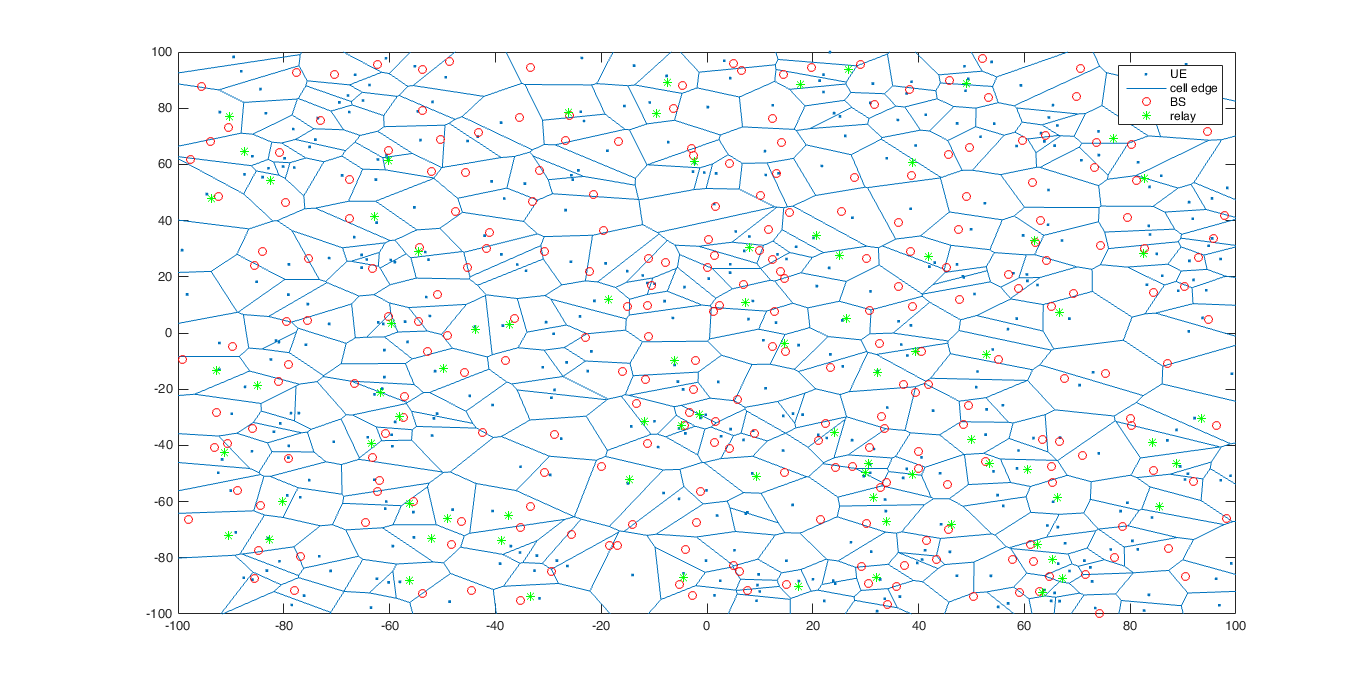
\includegraphics[height = 4in,width=7in,angle=00]{images/netLayoutSim.png}
\caption{\small Network Layout}
\label{fig:netLayoutSim}
\end{center}
\end{figure}
This a sample network layout generated by using the method discussed in previous subsection. We can see that some of the UEs are well within the range but have no BS. Only UEs with a BS are considered active. A fraction active UEs have relays, these UEs use PDF relaying. Cooperation probability = number of active UEs with relays/total number of active UEs.
\begin{figure}[H]
\begin{center}
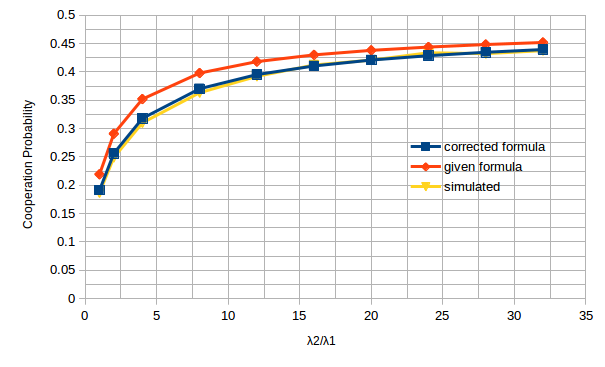
\includegraphics[height = 3in,width=4in,angle=00]{images/corrected.png}
\caption{\small Corrected cooperation probability of $E_3$}
\label{fig:correctedE3}
\end{center}
\end{figure}
In the published paper, the analytic result for cooperation probability of $E_3$ has an error. The correction being using $\mathcal{E}_3$ instead of $\mathcal{E}_2$ in eq.~\ref{eq:corrected}. The corrected analytic result matches the simulation result as can be seen in the above figure. 
\begin{figure}[H]
\begin{center}
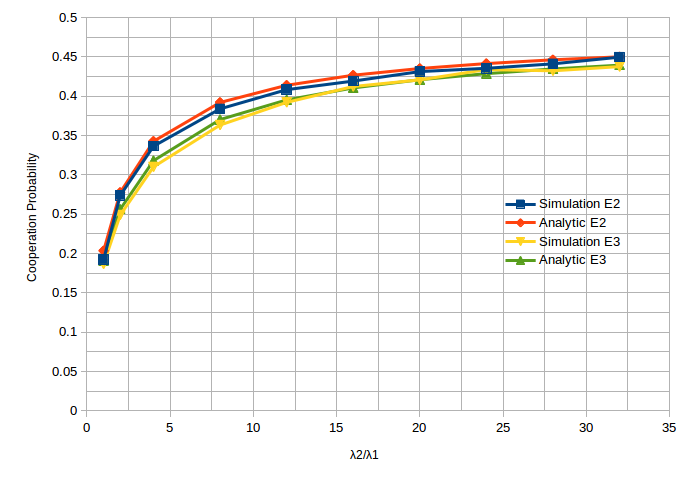
\includegraphics[height = 3in,width=4in,angle=00]{images/coopP.png}
\caption{\small Cooperation probabilities of $E_2$, $E_3$ versus user density ratio}
\label{fig:cooP}
\end{center}
\end{figure}
From the above graph we can see that cooperation probability of both policies increases with user density ratio($\lambda_2/\lambda_1$) and reach a maximum of 0.5 for very large user density ratio. Also, the analytic and simulations results closely match. 

\begin{figure}[H]
\begin{center}
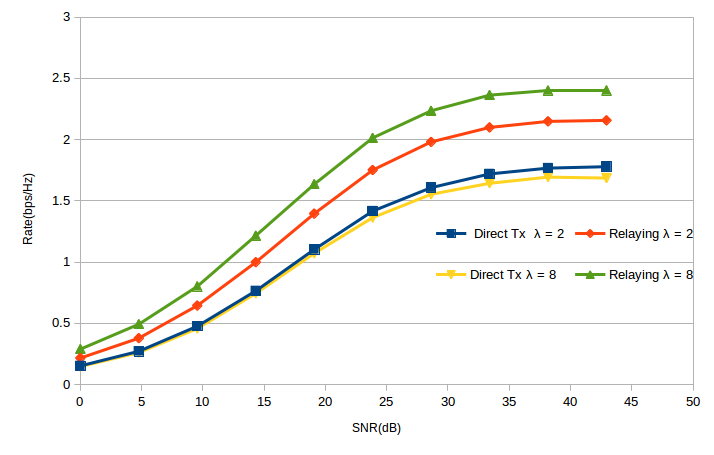
\includegraphics[height = 2.8in,width=4in,angle=00]{images/rates.png}
\caption{\small Average rate per user; $\lambda = \lambda_2/\lambda_1$}
\label{fig:rates}
\end{center}
\end{figure}
From the above figure, we can clearly see that average rate per user has increased when PDF relaying is deployed over the whole network. The rate also increases as user density ratio is increased but we caan't sure whether the rate keeps increasing with $\lambda$. It might happen that the rate decreases for very large user ratio density due to increase in interference.

\section{Downlink Cooperation Policy} \label{sec:downcoop}
A cooperation policy for downlink can be defined along the same lines as we did in uplink 
case. Let $P_b$ be the transmission power used by the base station and $P_r$ be relay power. A simple distance based policy would be
\begin{equation*}
	\{P_b r_1^{-\alpha} > P_b R_0^{-\alpha}, P_rr_2^{-\alpha} > P_bR_0^{-\alpha}\} 
\end{equation*}

\begin{figure}[h]
	\centering \vspace{-0.1in}

	\begin{tikzpicture}[scale=0.05]
		\coordinate [label=left:{\small $BS$}] (A) at (0,0);
		\fill [red,opacity=.5] (A) circle (50pt);

		\coordinate [label=right:{\small $U$}] (B) at (150,0);
		\fill [green,opacity=.5] (B) circle (50pt);

		\coordinate [label=above:{\small $Relay$}] (C) at (125,50);
		\fill [blue,opacity=.5] (C) circle (50pt);

		\draw (A) -- node[below=2pt] {\small $R_0$} (B) -- node[right=2pt] {\small $r_2$} (C)
												-- node[above=2pt] {\small $r_1$} cycle;

	\end{tikzpicture}

	\vspace{-10pt} \caption[Distances for Downlink Cooperation]{\small Distances for Downlink Cooperation}
	\label{fig:dwnlink}
\end{figure}

It can be rewritten as $\{ r_1 < R_0, r_2 < R_2 \}$ where $R_2 = cR_0, c = \big(\frac{P_r}{P_b}\big)^{\frac{1}{\alpha}} $ and $r_1, r_2$ are as defined in the figure \ref{fig:dwnlink}.  
The two conditions in the policy ensure that both BS-relay and relay-user links are stronger than BS-user link. The policy dictates that the idle user should be located in the shaded part of figure \ref{fig:region} to be considered for relaying.

\begin{figure}[h]
	\centering \vspace{0.1in}

	\begin{tikzpicture}[scale=0.015]
		\coordinate [label=left:{\small $BS$}] (A) at (0,0);
		\coordinate [label=right:{\small $U$}] (B) at (150,0);
		\fill [red,opacity=.5] (A) circle (200pt);
		\fill [green,opacity=.5] (B) circle (200pt);

		\draw (A) -- (B);
		\node (D) [name path=D,draw,circle through=(B)] at (A) {};
		%	\node (E) [name path=E,draw,circle(60)] at (B);
		% Name the coordinates, but do not draw anything:
		\draw (B) circle(120);
		\begin{scope}
			\clip (0,0) circle(150);
			\fill[blue,opacity=.5] (150,0) circle (120);
		\end{scope}
		%	\path [name intersections={of=D and E}];
	\end{tikzpicture}

	\vspace{-5pt} \caption[Feasible region]{\small Feasible region}
	\label{fig:region}
\end{figure}


Although interference and cooperation probabilities are not analysed for downlink case, we will study relay mobility for this case. The reason being, downlink case presents a more general geometrical region of interest as compared to uplink where both circles are of same radius and some of the results derived can be directly adapted to uplink case by changing the corresponding parameters. 



\chapter{Moving Relays}
\section{Mobility Model}
\subsection{Random Waypoint}

\section{Leaving in  one transition}
Let us find the probability with which a node at $(r,\theta)$ leaves the region in 
one transition. 
\subsection{Distances and Angles}
Consider the figure \ref{fig:rr1}. 
\begin{figure}[h]
    \centering \vspace{-0.1in}
    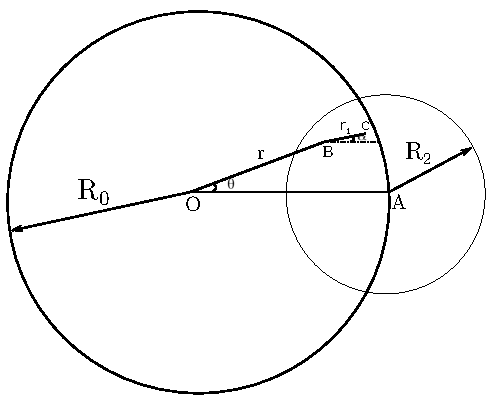
\includegraphics[width=0.6\textwidth]{images/geo1.pdf}
    \vspace{-20pt} \caption[Effect of the proximal Operator]{\small Effect of the Proximal Operator \footnotemark}
    \label{fig:rr1}
\end{figure}
\footnotetext{Image Source: \url{http://www.stanford.edu/~boyd/papers/pdf/prox_algs.pdf}}
The node starts at $B$ and let $C$ be 
the destination during first transition. $\alpha, r_1$ are chosen according to the mobility 
model described in the previous section. Whether or not $C$ is outside the region depends on
its distance from the circles' centers $O$ and $C$. $OC$ can be found using cosine rule:
$OC^2 = OB^2 + BC^2 - 2 \cdot OB \cdot BC \cdot \cos(\angle CBO)$. $\angle CBO = \pi-\theta+\alpha$ (see figure \ref{fig:ocac}).
\begin{figure}[h]
    \centering \vspace{-0.1in}
    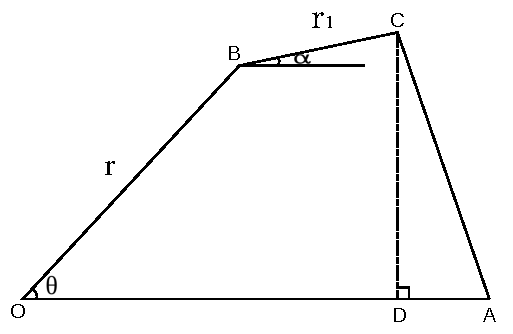
\includegraphics[width=0.6\textwidth]{images/geo2.pdf}
    \vspace{-20pt} \caption[Effect of the proximal Operator]{\small Effect of the Proximal Operator }
    \label{fig:ocac}
\end{figure}

 Therefore, \begin{equation} OC^2 = r^2 + r_1^2 + 2rr_1\cos(\theta-\alpha) \end{equation} To find $AC$, drop a perpendicular from $C$ to the line $OA$ and let the intersection point be $D$ as shown in figure \ref{fig:ocac}. Consider $\bigtriangleup CDA$, 
\begin{align*}
CD &= OB\sin\theta + BC\sin\alpha \\
&= r\sin\theta + r_1\sin\alpha \\
DA &= OA - OB\cos\theta - BC\cos\alpha \\
&= R_0-r\cos\theta-r_1cos\alpha
\end{align*}
Since $\angle CDA = \pi/2$, $AC^2 = CD^2 + DA^2$. $AC$ can therefore be given by 
\begin{equation}
	AC^2 = (r\sin\theta + r_1\sin\alpha)^2 + (R_0-r\cos\theta-r_1cos\alpha)^2
\end{equation}
To find which circle the node crosses first, we also need the angle made by the circle intersections at $B$. Let $\alpha_1$ and $\alpha_2$ be as shown in figures \ref{fig:alpha1} and \ref{fig:alpha2} where $BH$ is a horizontal line. 


\begin{figure}[h]
\centering \vspace{-0.1in}
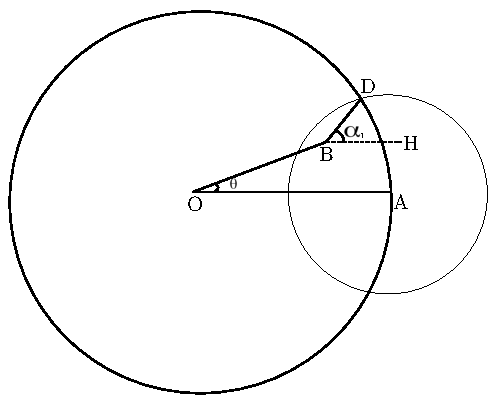
\includegraphics[width=0.6\textwidth]{images/geo3.pdf}
\vspace{-20pt} \caption[Effect of the proximal Operator]{\small Effect of the Proximal Operator }
\label{fig:alpha1}
\end{figure} 
\newpage
In figure \ref{fig:alpha1}, join $OD$ and drop
a perpendicular from $D$ to meet the extension of the $OB$ at $E$. To avoid clutter, let us 
remove the circles and form figure \ref{fig:alpha11}. 
\begin{figure}[h]
\centering \vspace{-0.1in}
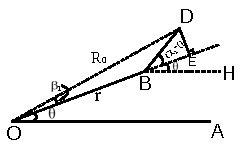
\includegraphics[width=0.6\textwidth]{images/geo4.pdf}
\vspace{-20pt} \caption[Effect of the proximal Operator]{\small Effect of the Proximal Operator }
\label{fig:alpha11}
\end{figure}
Consider $\bigtriangleup DOA$, 
\begin{align*}
	AD^2 &= OD^2 + OA^2 - 2 \cdot OD \cdot OA \cdot \cos(\beta_1+\theta) \\
	R_2^2 &= R_0^2 + R_0^2 - 2R_0^2\cos(\beta_1 + \theta)\\
\end{align*}
\begin{equation}\label{eq:beta1}
	\beta_1 = \cos^{-1}\bigg(1-\frac{R_2^2}{2R_0^2}\bigg) - \theta
\end{equation}
Using $\beta_1$ we can find $\alpha_1$
\begin{align*}
	\tan(\alpha_1 - \theta) &= \frac{DE}{BE} \\
							&= \frac{DE}{OE-OB}\\
							&= \frac{R_0 \sin\beta_1}{R_0\cos\beta_1 - r} \\
	\alpha_1 &= \theta + \tan^{-1}\bigg( \frac{R_0 \sin\beta_1}{R_0\cos\beta_1 - r}\bigg) \\
\end{align*}
\begin{figure}[h]
\centering \vspace{-0.1in}
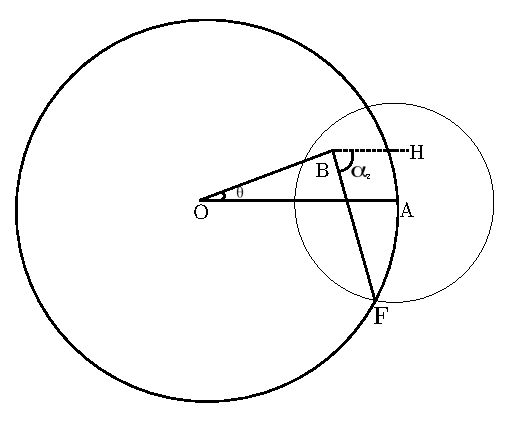
\includegraphics[width=0.6\textwidth]{images/geo5.pdf}
\vspace{-20pt} \caption[Effect of the proximal Operator]{\small Effect of the Proximal Operator }
\label{fig:alpha2}
\end{figure}
$\alpha_2$ and $\beta_2$ are defined in figures \ref{fig:alpha2} and \ref{fig:alpha21}. $\beta_2 = \beta_1 + \theta$ by symmetry. Using expression \ref{eq:beta1} for $\beta_1$, we get

\begin{equation}\label{eq:beta2}
	\beta_2 = \cos^{-1}\bigg(1-\frac{R_2^2}{2R_0^2}\bigg)
\end{equation}

\begin{figure}[h]
\centering \vspace{-0.1in}
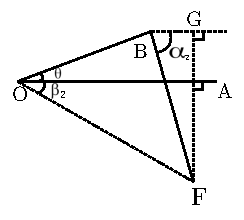
\includegraphics[width=0.6\textwidth]{images/geo6.pdf}
\vspace{-20pt} \caption[Effect of the proximal Operator]{\small Effect of the Proximal Operator }
\label{fig:alpha21}
\end{figure}

To find $\alpha_2$, consider $\bigtriangleup BGF$ in figure \ref{fig:alpha21}

\begin{align*}
 \tan\alpha_2 &= \frac{FG}{GB} \\
			  &= \frac{FA+AG}{GB} \\
			  &= \frac{R_0 \sin\beta_2 + r\sin\theta}{R_0 \cos\beta_2 - r\cos\theta} \\
\Rightarrow \alpha_2 &= \tan^{-1}\bigg( \frac{R_0 \sin\beta_2 + r\sin\theta}{R_0 \cos\beta_2 - r\cos\theta} \bigg) 
\end{align*}

\subsection{Probability}
When $-\alpha_2 < \alpha < \alpha_1$, $C$ is outside the region if $OC^2 > R_0^2$ and for other values of $\alpha$, the node leaves the region if $AC^2 > R_2^2$. The probability of node leaving the region in one transition, let us call it $\rho(r,\theta)$
, is given by
\begin{equation}\label{eq:prob1}
	\rho(r,\theta) = Pr(-\alpha_2 < \alpha < \alpha_1,OC^2 > R_0^2) + Pr(\alpha_1 < \alpha < 2\pi-\alpha_2, AC^2 > R_2^2) \\
\end{equation}
Let us rewrite the above in terms of $r_1$ whose distribution we know.
$AC^2 > R_2^2 \Rightarrow$

\begin{align*}
	(r\sin\theta + r_1\sin\alpha)^2 + (R_0-r\cos\theta-r_1cos\alpha)^2 &> R_2^2 \\
	r_1^2 \sin^2\alpha + r^2\sin^2\theta + 2rr_1\sin\theta\sin\alpha &+ \\ (R_0-r\cos\theta)^2 +
	r_1^2\cos^2\alpha - 2(R_0-r\cos\theta)r_1\cos\alpha - R_2^2 &> 0\\ 
	r_1^2 + 2 r_1 (r\sin\alpha\sin\theta-(R_0-r\cos\theta)\cos\alpha) + r^2\sin^2\theta +
	(R_0-r\cos\theta)^2 -R_2^2 &>0 \\
	r_1^2 + 2(r\cos(\theta-\alpha) - R_0\cos\alpha) r_1 + r^2\sin^2\theta +	(R_0-r\cos\theta)^2 - R_2^2 &> 0 
\end{align*}
The above inequality gives two feasible intervals for $r_1$ one of which is spurious since $r_1 > 0$ and the other is 
\begin{align}\label{ineq:ACcon}
	r_1 > (R_0\cos\alpha - r\cos(\theta-\alpha)) + \sqrt{\big(R_0\cos\alpha-r\cos(\theta-\alpha)\big)^2 + R_2^2 - r^2\sin^2\theta - 	(R_0-r\cos\theta)^2 }
\end{align}
Similar calculations as above will reduce $OC^2 > R_0^2$ to
\begin{align} \label{ineq:OCcon}
	r_1 > -r\cos(\theta-\alpha) + \sqrt{R_0^2 - r^2\sin^2(\theta-\alpha)}
\end{align}
Let us denote the R.H.S of the above two inequalities by $r_{12}$ and $r_{11}$ respectively.
Substituting \ref{ineq:ACcon} and \ref{ineq:OCcon} in \ref{eq:prob1}, we get
\begin{align*}
	\rho(r,\theta) &= Pr(-\alpha_2 < \alpha < \alpha_1,r_1 > r_{11}) + Pr(\alpha_1 < \alpha < 2\pi-\alpha_2, r_1 > r_{12}) \\
	&= \int_{-\alpha_2}^{\alpha_1} \int_{r_{\!_{11}}}^{\infty} f_{r_1,\alpha}(r_1,\alpha)dr_1 d\alpha +  \int^{2\pi-\alpha_2}_{\alpha_1} \int_{r_{\!_{12}}}^{\infty} f_{r_1,\alpha}(r_1,\alpha)dr_1 d\alpha  \\
	&= \int_{-\alpha_2}^{\alpha_1} f_{\alpha}(\alpha) \int_{r_{\!_{11}}}^{\infty} f_{r_1}(r_1)dr_1 d\alpha +  \int^{2\pi-\alpha_2}_{\alpha_1} f_{\alpha}(\alpha) \int_{r_{\!_{12}}}^{\infty} f_{r_1}(r_1)dr_1 d\alpha  \\
	&= \int_{-\alpha_2}^{\alpha_1} \frac{1}{2\pi} e^{-\lambda \pi r_{\!_{11}}^2} d\alpha +  \int^{2\pi-\alpha_2}_{\alpha_1} \frac{1}{2\pi} e^{-\lambda \pi r_{\!_{12}}^2} d\alpha
\end{align*}
\newpage
Putting it all together at one place for ease of reference, the probability with which a 
node at $(r,\theta)$ moves out of the region of interest during the next transition is 
\begin{equation} \label{eq:oneOutProb}
	\rho(r,\theta) = \int_{-\alpha_2}^{\alpha_1} \frac{1}{2\pi} e^{-\lambda \pi r_{\!_{11}}^2} d\alpha +  \int^{2\pi-\alpha_2}_{\alpha_1} \frac{1}{2\pi} e^{-\lambda \pi r_{\!_{12}}^2} d\alpha
\end{equation}
\\
Where
\begin{align*}
	r_{\!_{11}} &= -r\cos(\theta -\alpha) + \sqrt{R_1^2 - r^2\sin^2(\theta - \alpha)} \\
	&\\
	r_{\!_{12}} &= R_1 \cos \alpha - r\cos(\theta - \alpha)  +  \sqrt{[R_1 \cos \alpha - r\cos(\theta-\alpha) ]^2 - r^2\sin^2 \theta - [R_1 - r\cos \theta]^2 + R_2^2} \\
\end{align*}
\begin{align*}
	\beta_1 &= \cos^{-1}\bigg(1-\frac{R_2^2}{2R_0^2}\bigg) - \theta \\
	& \\
		\beta_2 &= \cos^{-1}\bigg(1-\frac{R_2^2}{2R_0^2}\bigg) \\
	& \\
	\alpha_1 &= \theta + \tan^{-1}\bigg( \frac{R_0\sin\beta_1}{R_0\cos\beta_1-r}\bigg)\\
			& \\
			\alpha_2 &= \tan^{-1}\bigg( \frac{r\sin\theta + R_0\sin\beta_2}{R_0cos\beta_2 - r\cos\theta} \bigg)
\end{align*}

\chapter{Mobility Markov Chain}
	The transitions in this mobility model have Markovian property in the sense that the next waypoint depends entirely on the current position. 
\begin{equation*}
	f_{X_n/X_{n-1},X_{n-2},\ldots,X_0}(x_n/x_{n-1},x_{n-2},\ldots,x_{0}) = f_{X_n/X_{n-1}}(x_n/x_{n-1})
\end{equation*}
Where $X_{n-1}$ is the current waypoint and $X_n$ is the next waypoint. \\
	The idea is to discretize the state space of this Markov chain and model the motion as an Absorbing Markov Chain in which the node transitions among the non-absorbing states present inside the region before finally moving to the absorbing state. 
Let the whole space be represented by $n+1$ states of which $n$ states lie inside the region of interest and the $n+1$th state represents the space outside the region. The transition probabilities among first $n$ states depend on the distances between the nodes and the transition probabilities from these $n$ states to the absorbing state is $\rho(r_i,\theta_i)$ where $(r_i,\theta_i)$ is the position of the $i$th state. We can then use the expressions given in \cite{wiki:markovWiki}
to find expected value and variance of the number of transitions a node makes before getting absorbed in the $(n+1)$th state. The transition probability matrix of this Markov Chain is  
\begin{equation*}
	P  = \left(
	\begin{array}{cc}
	Q & R \\
		\mathbf{0} & 1 \\
	\end{array} \right)
\end{equation*}
	Where $Q_{n \times n}$ is the transition probability matrix of $n$ non-absorbing states and $R_{n\times1}$ contains the probabilities of moving out in one step from each of those $n$ states. 
	 $\mathbf{t}_{n \times 1}$, the vector which contains expected number of transitions, is given by
\begin{equation*}
	\mathbf{t} = A\mathbf{1} \\
\end{equation*}
and the variance vector $V$ is given by
\begin{equation*}
	 V = (2A-I)\mathbf{t} - \mathbf{t}_{sq}
\end{equation*}
where $A = \sum_{k=0}^{\infty} Q^k = (I-Q)^{-1}$ is the fundamental matrix.

	It remains to be seen how well this model works.

\chapter{Simulations and Results}
For all simulations, a 1000x1000 square is used to represent the whole 2-D plane. This size is good enough in the sense that using a larger square led to longer runtimes with little to no 
effect on the results. In the mobility model we used, transition length is Rayleigh distributed. To draw a length from Rayleigh distribution, the following method is used:

\begin{enumerate}
	\item Draw a number N from Poisson distribution with density $\lambda A$ where $A$ is the area of the square.
	\item Distribute these N points uniformly on the square 
	\item Of these N points, choose the point that is closest to the point under consideration. 
\end{enumerate}

As discussed in \cite{ganti}, this leads to Rayleigh distribution of transition length and can be proved easily using null probability of a Poisson Point Process. 

\section{$E[L]$}
To test if the above mentioned method introduces any artefacts, let us see how simulated $E[L]$ fares with the formula $E[L] = \frac{1}{2\sqrt{\lambda}}$. Simulated expected length is calculated by averaging transition lengths of 100 traces in each of which the node makes 1000 transitions. 
\begin{figure}[h]
	\centering \vspace{-0.1in}
	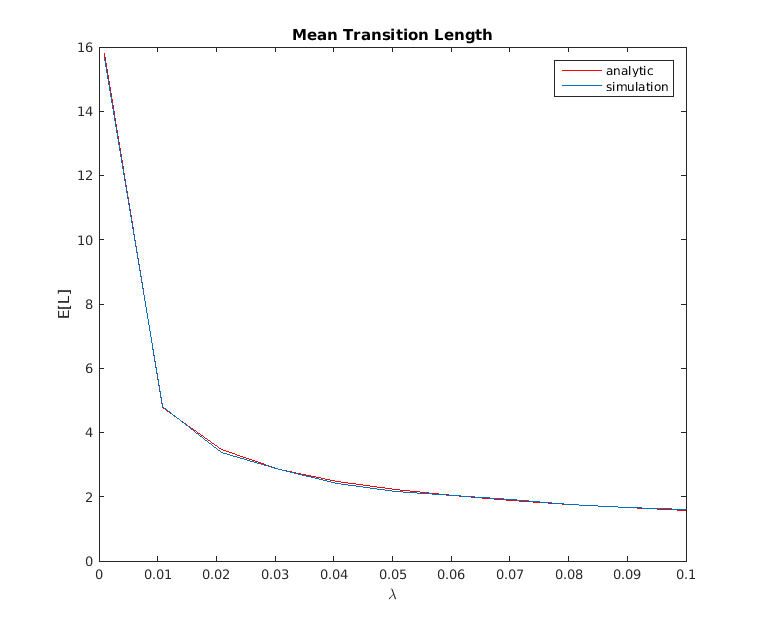
\includegraphics[width=0.75\textwidth]{images/rwpStat.png}
	\vspace{-20pt} \caption[Mean transition length vs. $\lambda$]{Mean transition length vs. $\lambda$}
	\label{fig:rwpEL}
\end{figure}
As seen in the graph \ref{fig:rwpEL}, the simulated value closely follows the analytical formula.
\section{$\rho(r,\theta)$}
In this section we look at how the probability $\rho(r,\theta)$ of moving out in one step varies in the region i.e., for different $r$ and $\theta$ and with the mobility parameter $\lambda$. 

\subsection{$\rho(r,\theta)$ vs. $\lambda$}

The plots in figure \ref{fig:vslambda} are for points inside the region and along the line joining centers of circles. At each iteration the node is placed at $(r,0)$ and a PPP($\lambda$) is generated. Probability is calculated by taking expected value of the indicator random variable which takes value 1 if the nearest point in PPP is outside the region and 0 if it is inside the region. 
\begin{figure}[ht!]
     \begin{center}
%
        \subfigure[$\lambda = 0.0005$]{%
            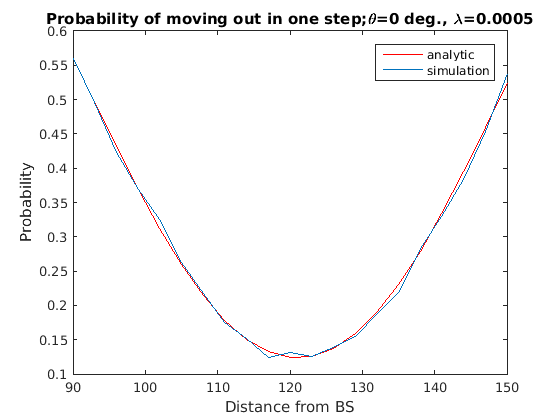
\includegraphics[width=0.6\textwidth]{images/oneOutProbl0005t0.png}
        }%
        \subfigure[$\lambda = 0.001$]{%
           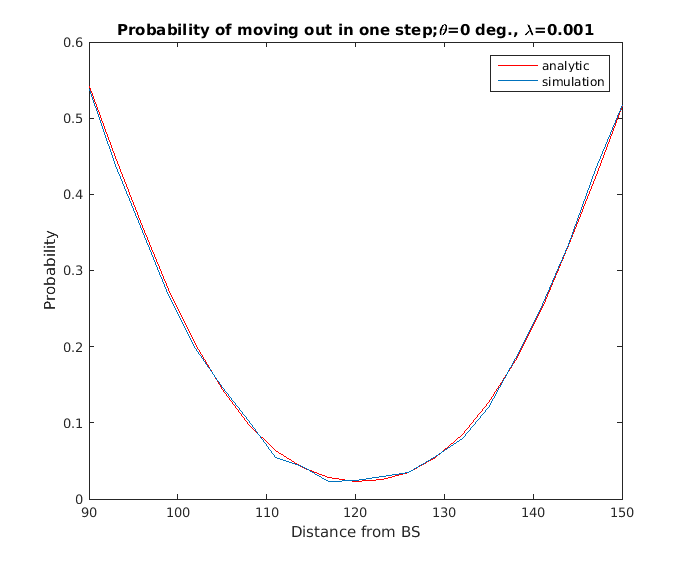
\includegraphics[width=0.55\textwidth]{images/oneOutProbl001t0.png}
        }\\ %  ------- End of the first row ----------------------%
        \subfigure[$\lambda = 0.005$]{%
            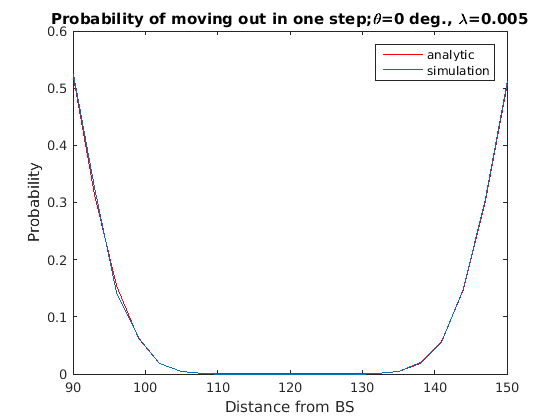
\includegraphics[width=0.6\textwidth]{images/oneOutProbl005t0.png}
        }%

%        \subfigure[Caption of Fourth Figure]{%
%            \label{fig:fourth}
%            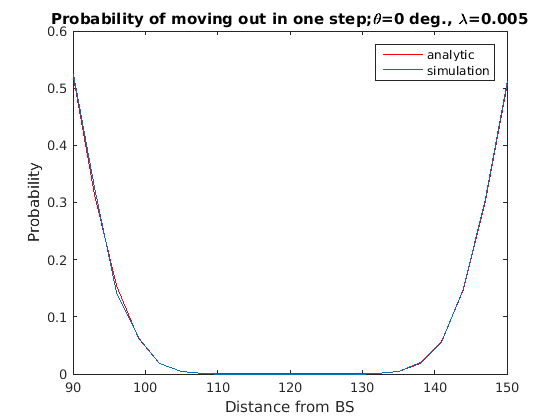
\includegraphics[width=0.4\textwidth]{images/oneOutProbl005t0.png}
        %}%
%
    \end{center}
	\caption[$\rho(r,0)$ vs. $\lambda$]{\small $\rho(r,0)$ vs. $ \lambda$}%
   \label{fig:vslambda}
\end{figure}
What we can observe in figure \ref{fig:vslambda} is that the probability for the points well within the region decreases as $\lambda$ is increased. For points near the boundary of the region, the probability doesn't change significantly. This is in line with what is expected. For points well inside the region, $E[L]$ primarily decides whether or not they leave the region and for points closer to the boundary, the probability depends on the choice of angle $\alpha$.
\subsection{$\rho(r,\theta)$ for different $\theta$}
\begin{comment}
\begin{figure}[h]
	\centering \vspace{-0.1in}
	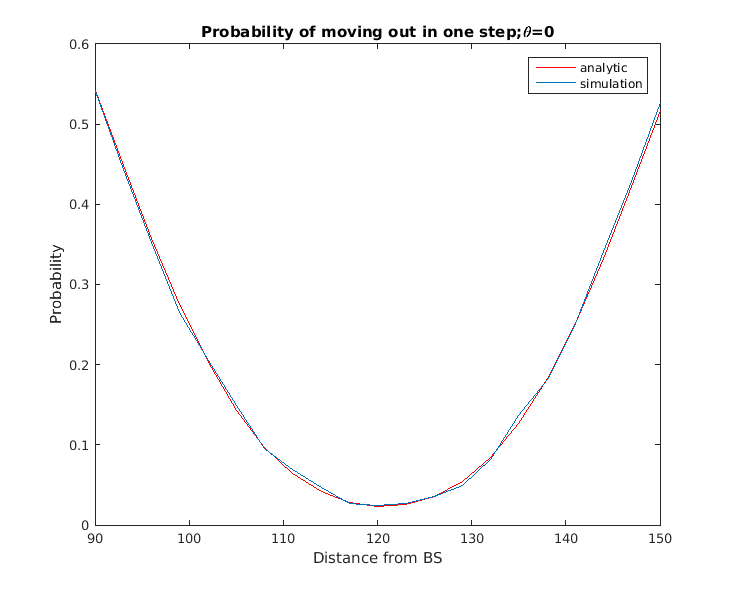
\includegraphics[width=0.75\textwidth]{images/oneOutProb0.png}
	\vspace{-20pt} \caption[Effect of the proximal Operator]{\small Effect of the Proximal Operator }
	\label{fig:oneOut0}
\end{figure}

\begin{figure}[h]
	\centering \vspace{-0.1in}
	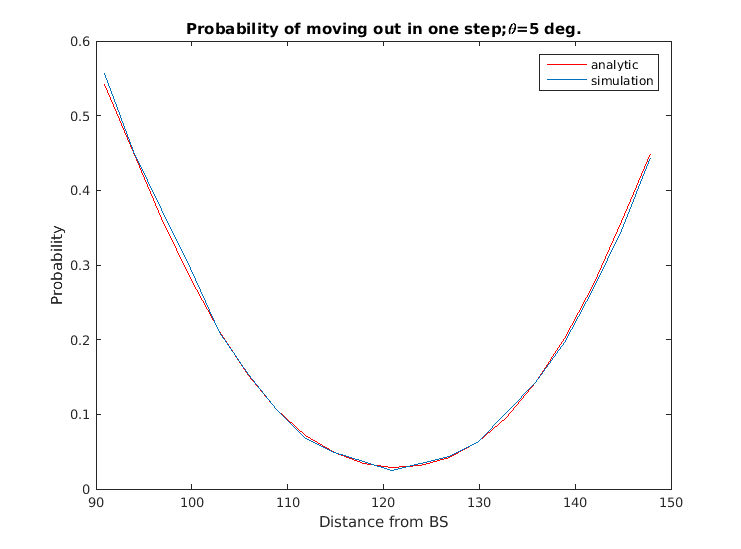
\includegraphics[width=0.75\textwidth]{images/oneOutProb5.png}
	\vspace{-20pt} \caption[Effect of the proximal Operator]{\small Effect of the Proximal Operator }
	\label{fig:oneOut5}
\end{figure}

\begin{figure}[h]
	\centering \vspace{-0.1in}
	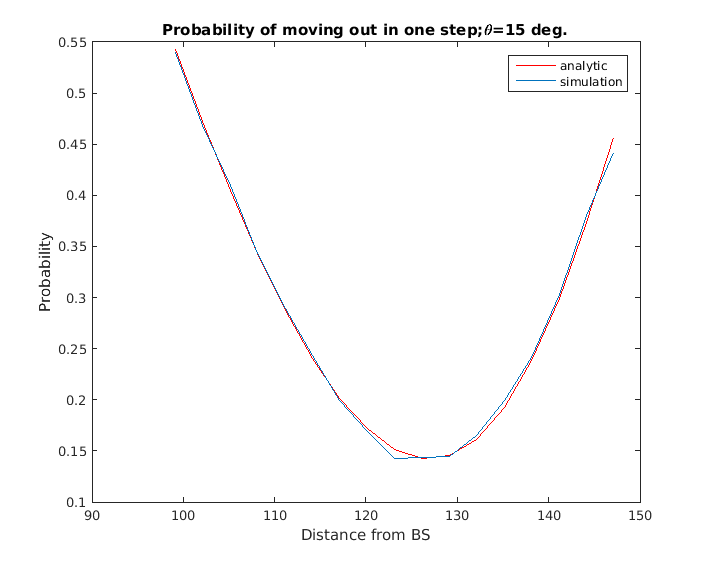
\includegraphics[width=0.75\textwidth]{images/oneOutProb15.png}
	\vspace{-20pt} \caption[Effect of the proximal Operator]{\small Effect of the Proximal Operator }
	\label{fig:oneOut15}
\end{figure}

\begin{figure}[h]
	\centering \vspace{-0.1in}
	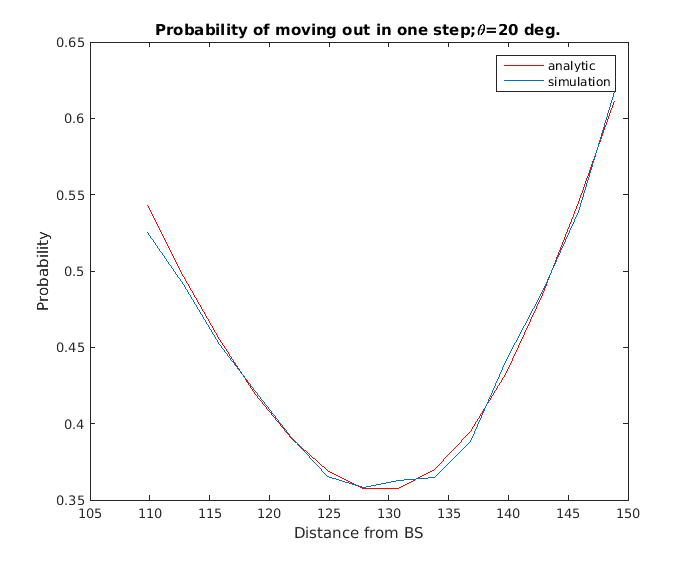
\includegraphics[width=0.75\textwidth]{images/oneOutProb20.png}
	\vspace{-20pt} \caption[Effect of the proximal Operator]{\small Effect of the Proximal Operator }
	\label{fig:oneOut20}
\end{figure}
\end{comment}

Figure \ref{fig:vangles} shows how $\rho(r,\theta)$ along the radius changes with $\theta$. We can see that it increases with $\theta$ for points inside the region and doesn't change significantly for points at the edges. We can see that the maximum can occur at both edges.

\begin{figure}[H]
     \begin{center}
%
		 \subfigure[$\theta = 0^{\circ}$]{%
            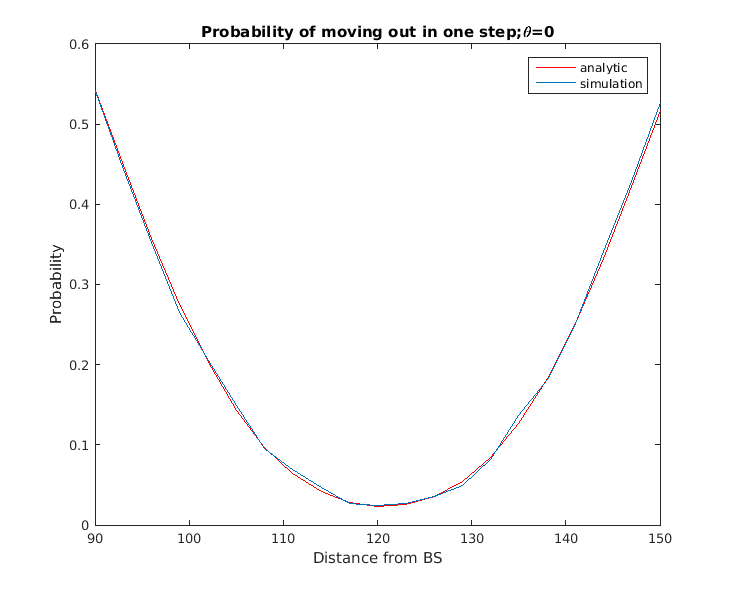
\includegraphics[height = 2.5in,width=3.5in]{images/oneOutProb0.png}
        }%
        \subfigure[$\theta = 5^{\circ}$]{%
           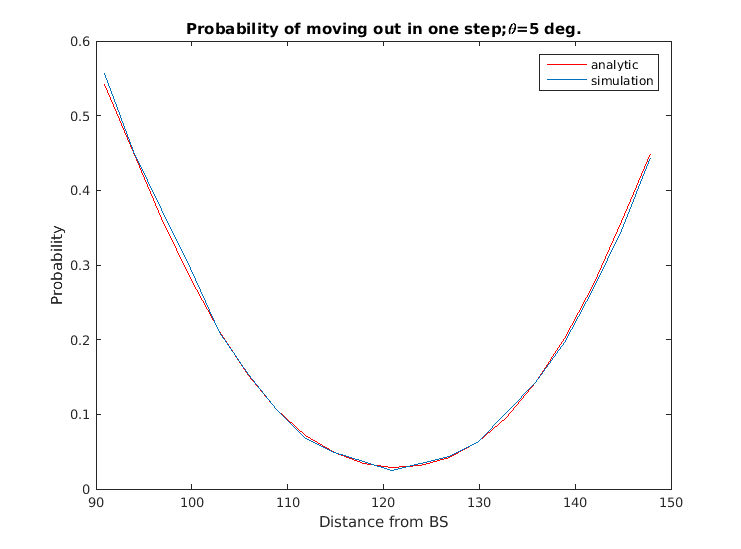
\includegraphics[height = 2.5in,width=3.5in]{images/oneOutProb5.png}
        }\\ %  ------- End of the first row ----------------------%
        \subfigure[$\theta = 15^{\circ}$]{%
            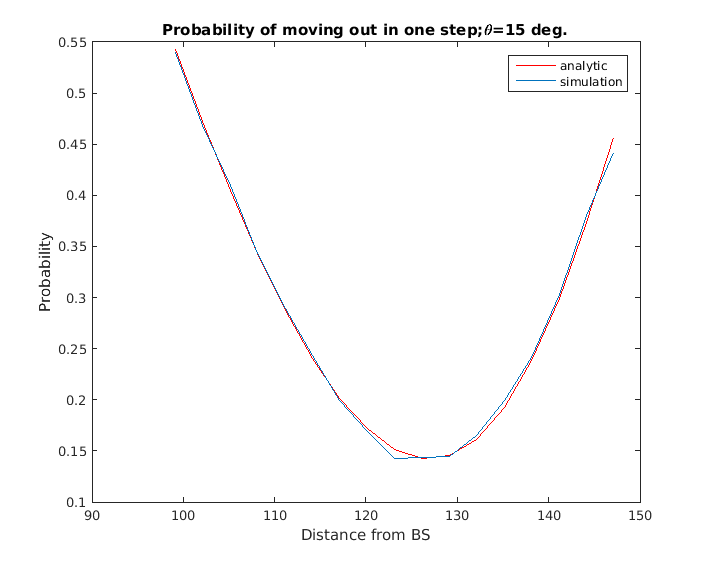
\includegraphics[height = 2.5in,width=3.5in]{images/oneOutProb15.png}
        }%

        \subfigure[$\theta = 20^{\circ}$]{%
            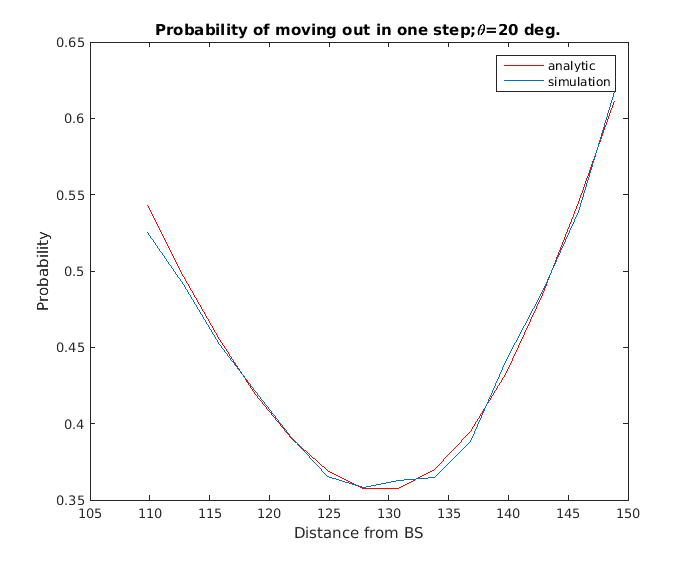
\includegraphics[height = 2.5in,width=3.5in]{images/oneOutProb20.png}
        }%
%
    \end{center}
	\caption[$\rho(r,\theta)$ at different angles]{$\rho(r,\theta)$ at different angles}%
   \label{fig:vangles}
\end{figure}
\section{E[N]}
Figure \ref{fig:EN} shows the expected number of steps in which a node leaves the region.
The plots are for points along the radius at angles $\theta = 10^{\circ}$ and $\theta = 15^{\circ}$. We can see that the analytical formula agrees better for narrower regions. As discussed in Chapter 4, this can be improved by modelling the motion of a node as an absorbing Markov Chain and discretizing the state space.

\begin{figure}[ht!]
     \begin{center}
%
		 \subfigure[$\theta = 10^{\circ}$]{%
            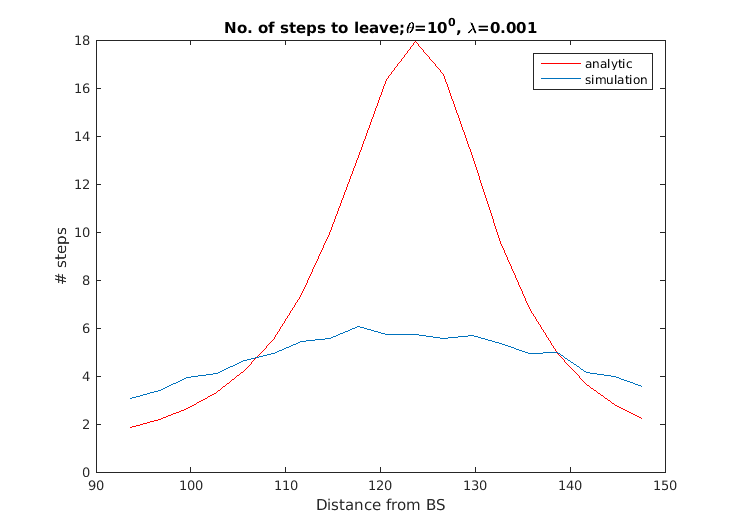
\includegraphics[height = 2.5in,width=3.5in]{images/stepst10.png}
        }%
        \subfigure[$\theta = 15^{\circ}$]{%
           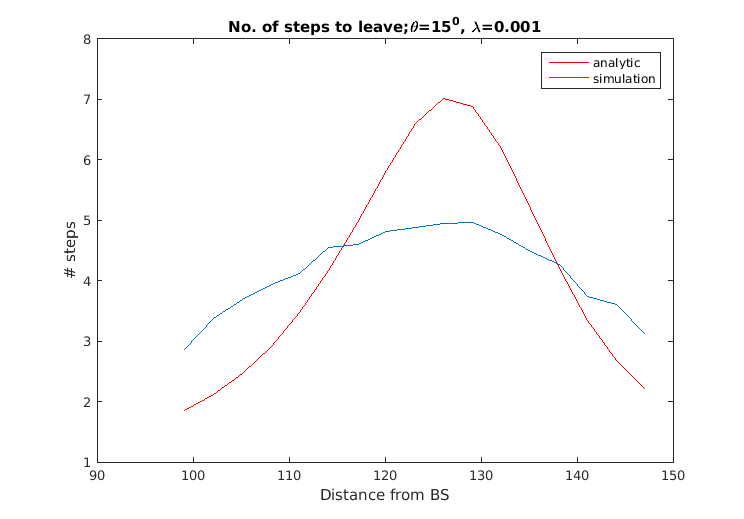
\includegraphics[height = 2.5in,width=3.5in]{images/stepst15.png}
        }\\ %  ------- End of the first row ----------------------%
%
    \end{center}
	\caption[Expected number of transitions]{Expected number of transitions}%
   \label{fig:EN}
\end{figure}






\chapter{Conclusion and Further Work}
\section{Conclusion}
Based on the results obtained we conclude the following:
\begin{enumerate}
\item Based on the work of H. Elkotby, we verified that there is throughput gain when user-assisted relaying is deployed in cellular network despite the increase in interference. 
\item The probability of leaving the region is maximum for points on the boundary. The maximum shifts to right side border for points closer to intersection of circles.
\item The expected number of transitions can be better approximated by discretizing the region as states in a Markov Chain.
\end{enumerate}

\section{Further Work}
The following can be looked at in the future.
\begin{enumerate}
\item	Using the idea presented in chapter 4 to obtain lower and upper bounds on the expected number of steps if not to find the the value itself to a close apprximation.
\item	Through out the work we took $R_0$, the distance between base station and user, to be constant and did not assume the distribution of inital position of the relay. The distributions of $R_0$ and initial position can be incorporated to find the effect of mobility on the whole network.
\item	To include sojourn time as one of the deciding parameters in relay selection.     
\item	To apply the general methodology used in this work for other mobility models. 
\end{enumerate}


\singlespace 
\bibliographystyle{ieeetr}
%\nocite{*}
\addcontentsline{toc}{chapter}{Bibliography}
\bibliography{bib}
% \newpage
% \clearpage
% \vspace*{-12pt}\addcontentsline{toc}{chapter}{Index}
\printindex


\end{document}
